\documentclass[11pt]{article}

\usepackage[margin=2.5cm]{geometry}
\usepackage{fontspec}
\usepackage{xeCJK}
\setCJKmainfont{Batang}[BoldFont=Malgun Gothic, AutoFakeSlant=0.15]
\setCJKsansfont{Malgun Gothic}
\xeCJKsetup{CJKspace=true}
\XeTeXlinebreaklocale "ko"
\XeTeXlinebreakskip = 0pt plus 1pt minus 1pt

\usepackage{amsmath}
\usepackage{amssymb}
\usepackage{booktabs}
\usepackage{tabularx}
\usepackage{array}
\usepackage{parskip}
\usepackage{graphicx}
\usepackage[section]{placeins}
\usepackage{tikz}
\usepackage[colorlinks=true,linkcolor=blue,urlcolor=blue,citecolor=blue]{hyperref}

\renewcommand{\figurename}{그림}
\renewcommand{\tablename}{표}
\renewcommand{\contentsname}{목차}
\renewcommand{\abstractname}{초록}
\renewcommand{\refname}{참고문헌}
\renewcommand{\appendixname}{부록}

\newcolumntype{Y}{>{\raggedright\arraybackslash}X}
\newcommand{\E}{\mathbb{E}}
\newcommand{\N}{\mathcal{N}}
\newcommand{\R}{\mathbb{R}}
\newcommand{\code}[1]{\texttt{#1}}

\title{전역·국소·하이브리드 잠재:\\계층적 메시 GNN 위의 일대다 대체 모델\\HI-MGN-V와 cHI-MGNflow}
\author{AI-CAE4ALL 기술 리포트\
  \small\code{methods/MeshGraphNets\_Variational}, \code{methods/HI\_MGNFlow}}
\date{2026-10-12 (2026-09-18판 전면 개정)}

\begin{document}
\maketitle

\begin{abstract}
같은 형상·같은 하중이 하나가 아닌 여러 응답을 낳는 문제가 있다. 원통
셸의 좌굴처럼, 입력에 나타나지 않는 미세한 초기 결함이 어느 분기로 갈지를
정하는 경우다. 결정론적 메시 GNN은 이런 문제에서 분기들의 평균, 즉 어떤
실제 표본과도 닮지 않은 필드를 내놓는다. 본 리포트는 같은 계층적 메시
GNN(HI-MGN V-cycle) 위에서 \textbf{잠재 변수를 어디에 두는지만} 다른 두
생성 대체 모델을 코드 수준에서 기술하고 비교한다.
\textbf{HI-MGN-V}는 그래프당 하나인 96차원 잠재를 AdaLN-Zero로 V-cycle의
모든 블록에 공간적으로 균일하게 주입한다(전역).
\textbf{cHI-MGNflow}는 LDGN(Lino, Pfaff \& Thuerey, ICLR 2025)의 2단계
설계를 따라 가장 coarse한 레벨의 노드마다 4채널 잠재($256\times4$)를 두고,
그 위에서 flow-matching prior를 학습한다(국소). 기본 prior는 4-hop
수용영역의 국소 GNN이다. 선택 옵션인 전역 토큰(\code{prior\_global token})은
\emph{prior 내부에만} 그래프 단위 결합을 더하고, 잠재와 디코더는 국소로
남긴다(하이브리드).
원통 셸 좌굴 데이터셋(학습 150 형상 $\times$ 결함 64 표본, 입력은 결함 없는
공칭 형상)에서 형상당 1000 표본으로 평가했다. cHI-MGNflow는 평균을
맞추지만(평균비 1.02) 퍼짐이 부족하다(sd비 0.66). HI-MGN-V는 진폭이 작고
(평균비 0.83) 잘못된 분기에 질량을 둔다. test의 W1/sd는 0.69 대 1.38이다.
진단 실험은 두 실패의 원인이 다름을 보인다. HI-MGN-V는 인코더가 표본 간
변동의 절반 정도만 잠재에 담는다. 같은 디코더에서 $z$를 직접 최적화하면
설명 비율이 0.85까지 오른다. cHI-MGNflow는 posterior가 정확하지만(sd비
0.97), 국소 prior가 노드 사이의 결합을 잃는다. 좌표별 분산은 맞지만 상위
주성분 방향의 분산은 0.4--0.5배다. 이 결과가 전역 토큰을 추가한 동기이며,
토큰 실험은 아직 진행 중이다.
\end{abstract}

\tableofcontents

%======================================================================
\section{서론}\label{sec:intro}

MeshGraphNets(MGN) 계열 모델은 encode--process--decode 구조로 메시 위의
물리량을 결정론적으로 예측한다~\cite{pfaff2021}. 이 구조는 입력이 응답을
유일하게 정하는 문제를 전제한다. 그러나 응답이 입력에 나타나지 않는
요인에 따라 갈리는 문제가 있다. 원통 셸의 축압축 좌굴이 대표적이다. 같은
공칭 형상, 같은 하중이라도 수십 $\mu$m 수준의 초기 결함이 좌굴 여부와
모드를 정한다. 이때 회귀 손실로 학습한 모델은 분기들의 조건부 평균
$\E[y\mid c]$로 수렴하고, 그 평균 필드는 어떤 실제 표본과도 닮지 않는다.
필요한 것은 조건부 분포 $p(y\mid c)$에서 표본을 뽑는 모델이다.

그림~\ref{fig:diag-setup}(a,b)가 이 상황을 보여준다. 형상 g5($R=158.6$,
$t=1.61$, $L=206.2$, $\Delta=1.02$\,mm, $\lambda=0.80$)에서 64개 결함 표본 중
16개는 최대 변위가 4\,mm를 넘고 나머지는 1\,mm 근처에 머문다. 모델이 보는
입력은 64개 모두 같다.

이 문제에 대해 Lino, Pfaff \& Thuerey~\cite{lino2025}는 DGN(필드 공간의
diffusion graph network)과 LDGN(압축된 잠재 공간의 diffusion)을 제안했다.
LDGN의 핵심은 두 단계다. 먼저 그래프 오토인코더로 필드를 coarse 노드별
잠재로 압축하고, 그다음 그 잠재 위에서만 생성 prior를 학습한다. 본
리포트는 이 관점을 계층적 MGN 위로 옮기면서 하나의 설계 질문에 집중한다.

\begin{quote}
\textbf{잠재 변수를 어디에 둘 것인가.} 그래프 전체에 하나(전역)인가,
coarse 메시 노드마다(국소)인가, 노드마다 두되 prior가 전역적으로 결합하는
형태(하이브리드)인가.
\end{quote}

\paragraph{분류 요약.} 코드와 대조한 세 모델의 분류는 다음과 같다(\S\ref{sec:compare}, 표~\ref{tab:three-designs}).
\begin{itemize}
\item \textbf{HI-MGN-V --- 전역.} 잠재 $z\in\R^{3\times32}$가 그래프당
  하나다. 레벨별 슬롯 $z_l$이 그 레벨의 모든 노드에 같은 변조를 준다.
\item \textbf{cHI-MGNflow, 기본(\code{prior\_global none}) --- 국소.} 잠재
  $z\in\R^{|V_L|\times C}=\R^{256\times4}$이다. prior는 $G_L$ 위의 평탄한
  GnBlock 4개로, 수용영역이 4 hop이다. $G_L$의 지름은 18 hop이다. 디코더도
  국소적인 V-cycle 상승 경로다.
\item \textbf{cHI-MGNflow, \code{prior\_global token} --- 하이브리드.}
  2026-10-06(커밋 \code{5b61f5b})에 추가된 선택 옵션이다. 잠재와 디코더는
  국소 그대로이고, \emph{prior의 velocity 네트워크 안에서만} 그래프당 전역
  토큰 하나가 256개 coarse 노드를 결합한다. 체크인된 ex3 baseline 설정은 이
  키를 쓰지 않으므로 기본값 \code{none}(국소)이다. 토큰은
  \code{b300\_sweep}의 \code{tok*} 계열 arm에서만 켜져 있다.
\end{itemize}
즉 ``HI-MGN-V는 전역, 기존 cHI-MGNflow는 국소, 현재 cHI-MGNflow는
하이브리드''라는 구분은 맞다. 단, 하이브리드는 \textbf{prior에만} 해당하고
옵션이다.

\paragraph{기여.}
\begin{enumerate}
\item 같은 V-cycle 위에 전역/국소/하이브리드 잠재를 두는 두 모델을 구현과
  일치하는 수준으로 정식화한다(\S\ref{sec:backbone}--\ref{sec:token}).
  2026-09-18판의 오기(AdaLN-Zero의 ``항등 초기화'', 추론 비용 ``V-cycle
  2회'', spread 지표의 정의, LDGN에 대한 서술 등)를 바로잡았다
  (부록~\ref{app:errata}).
\item 원통 셸 좌굴 벤치마크와, 형상당 1000 표본·FEA 표본 노이즈 바닥을 쓰는
  평가 프로토콜을 정리한다(\S\ref{sec:exp}).
\item 두 모델의 실패를 분리하는 진단을 제시한다. posterior와 prior를 같은
  고정 디코더로 비교하고, $z$ 최적화와 shuffle/coherent 대조를 쓴다.
  HI-MGN-V는 인코더 병목, cHI-MGNflow는 prior의 노드 간 결합 부족이 주원인이다.
\end{enumerate}

\begin{figure}[!htbp]
\centering
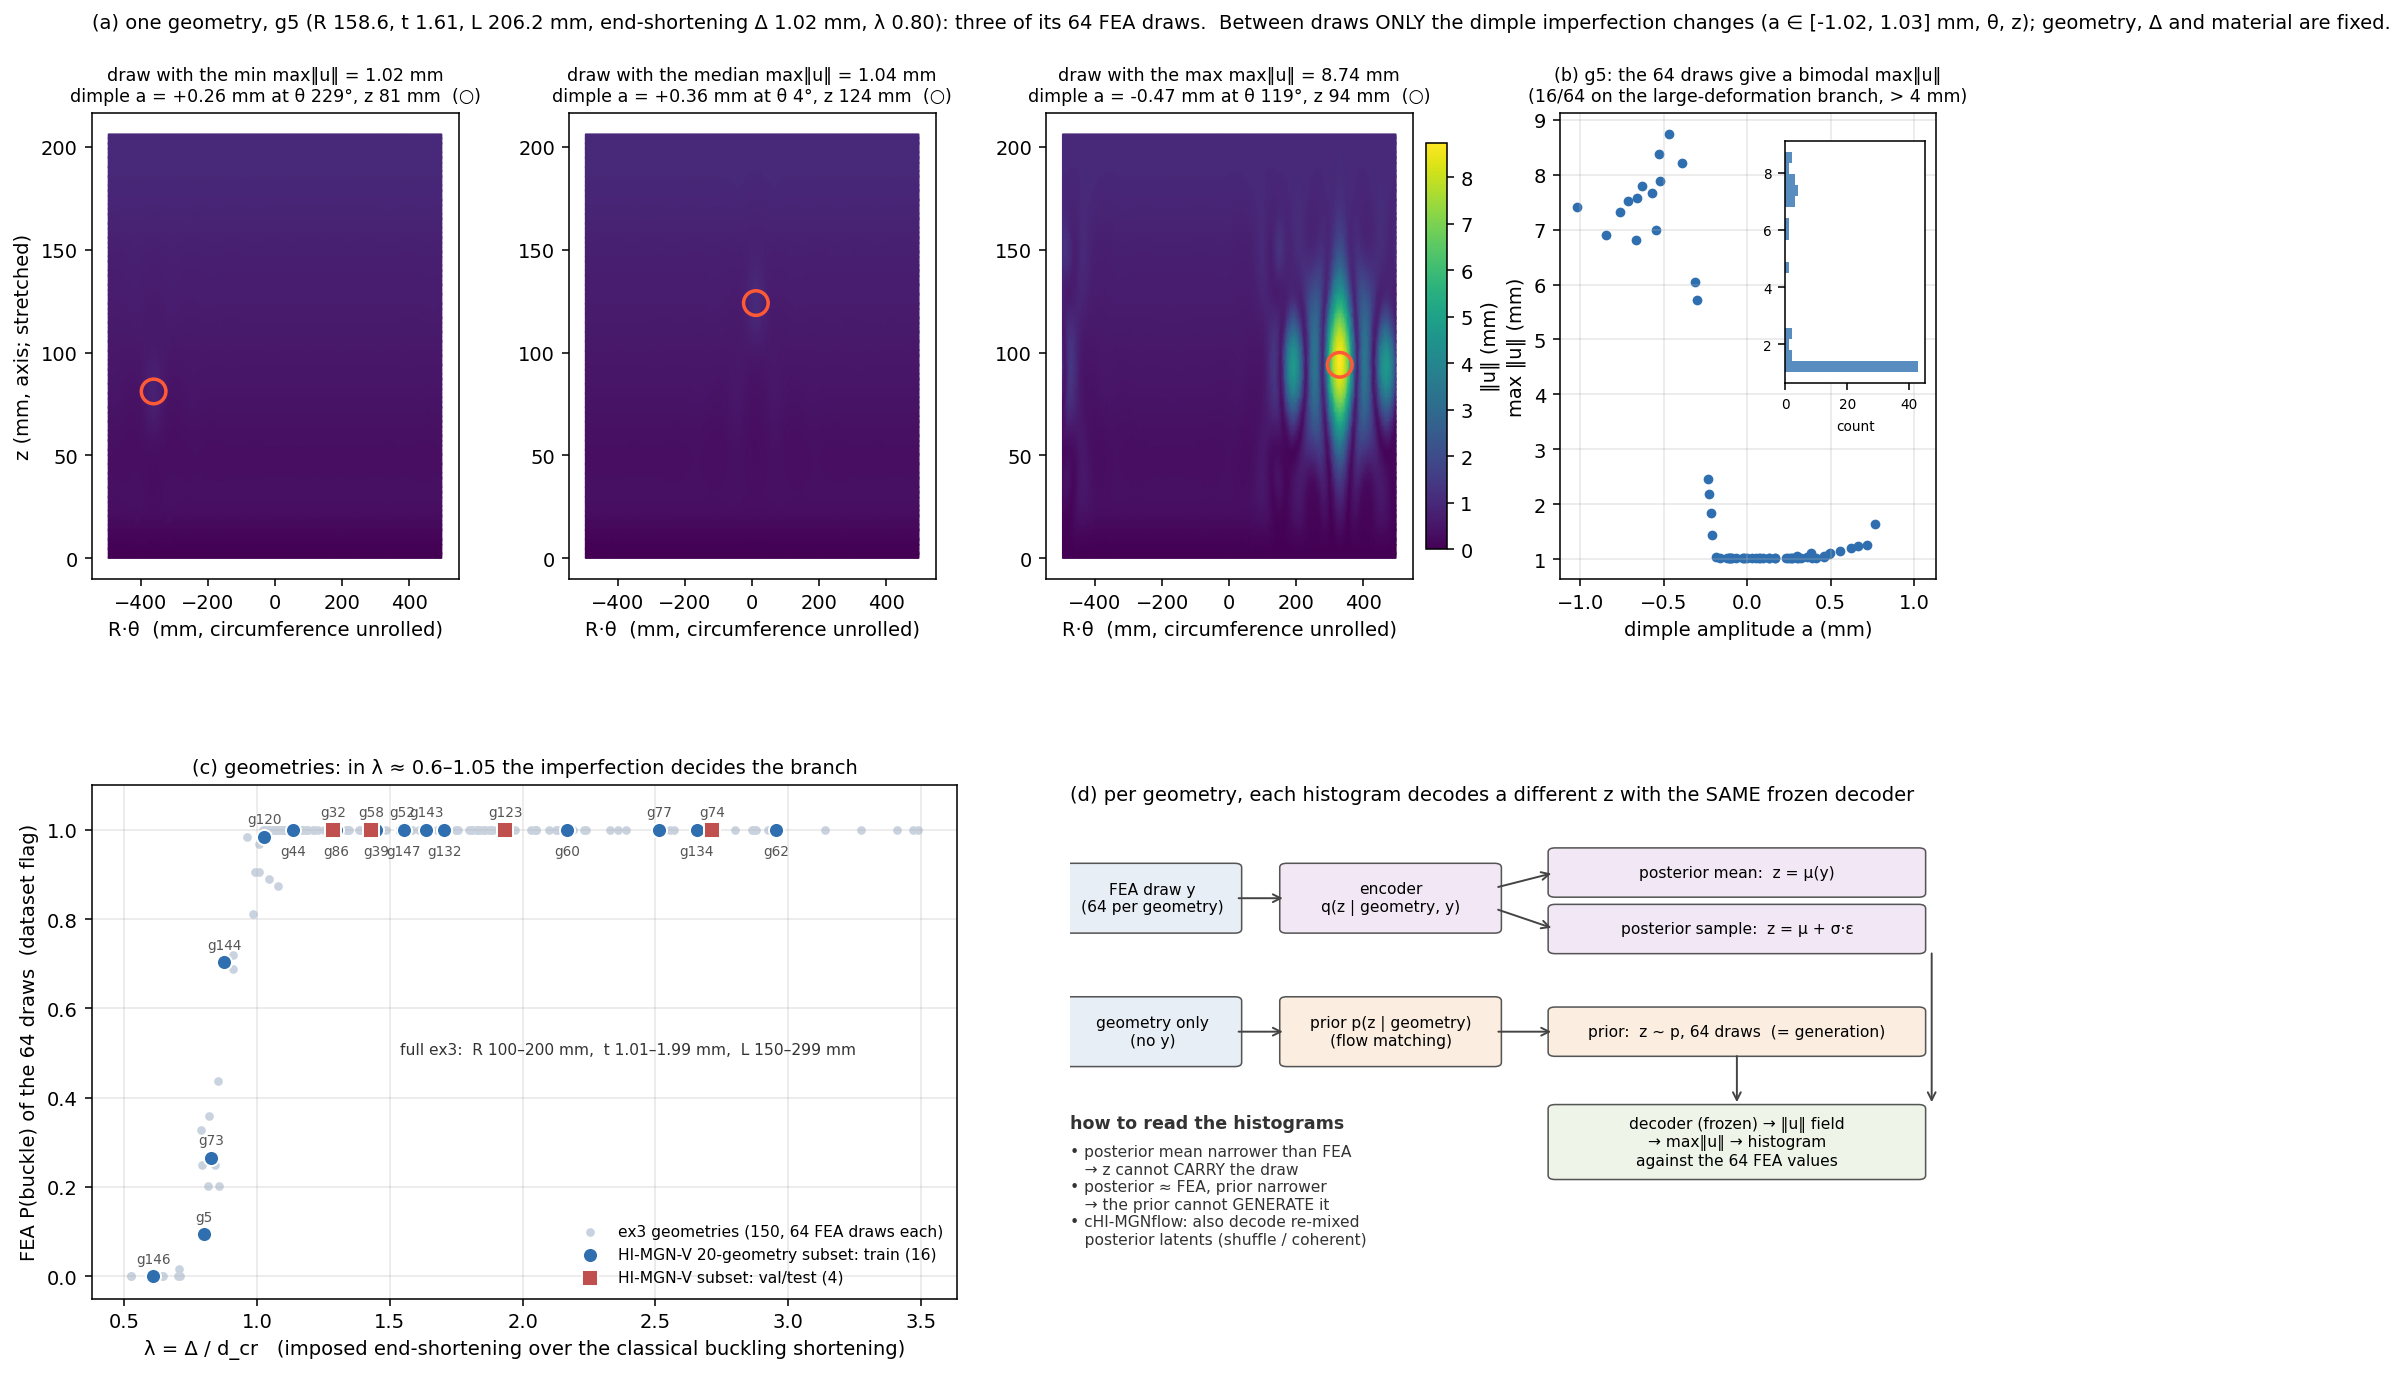
\includegraphics[width=\linewidth]{figures/diag_setup.png}
\caption{일대다 문제와 진단 절차. (a) 형상 g5의 FEA 표본 세 개
  (최소·중앙·최대; 최대 변위 1.02 / 1.04 / 8.74\,mm). 세 표본의 모델 입력은
  같다. (b) g5의 64개 표본에 대한 최대 $\|u\|$ 대 결함 진폭 $a$. 분포가
  양봉이며, 16/64가 4\,mm를 넘는다. (c) 학습 150 형상 전체의 FEA 좌굴 확률
  $P(\text{buckle})$ 대 하중비 $\lambda$. 표시된 점은 HI-MGN-V 부분실험에 쓴
  20개 형상이다(학습 16, 검증/시험 4: g32, g58, g123, g74). (d) 진단
  절차(\S\ref{sec:diag-v}, \S\ref{sec:diag-chi}). posterior 평균, posterior
  표본, prior 표본을 같은 고정 디코더로 디코딩해 FEA 히스토그램과 비교한다.}
\label{fig:diag-setup}
\end{figure}

%======================================================================
\section{관련 연구}\label{sec:related}

\paragraph{메시 GNN과 멀티스케일.} MGN~\cite{pfaff2021}은 메시 위의 메시지
패싱으로 시뮬레이션을 학습한다. 깊이가 고정된 메시지 패싱은 수용영역이
hop 수에 묶인다. 이를 넘기 위해 MS-MGN~\cite{fortunato2022}은 2-레벨 계층을,
BSMS-GNN~\cite{cao2023}은 bi-stride 풀링 계층을 도입했다. 본 리포트의
백본(HI-MGN)은 FPS 시드와 BFS Voronoi 셀로 계층을 만들고, U-Net형 V-cycle로
레벨 사이를 오간다(\S\ref{sec:backbone}).

\paragraph{변분 오토인코더.} VAE~\cite{kingma2014}와 그래프 버전
VGAE~\cite{kipf2016}는 posterior $q(z\mid y)$와 고정 prior $\N(0,I)$를 KL로
맞춘다. InfoVAE~\cite{zhao2019}는 KL 대신 집계 posterior와 prior 사이의
MMD~\cite{gretton2012}를 쓴다. HI-MGN-V는 MMD를 쓰고, 학습된 조건부 prior를
따로 둔다.

\paragraph{DGN과 LDGN.} Lino, Pfaff \& Thuerey~\cite{lino2025}는 메시 위의
조건부 분포 학습을 diffusion으로 다룬다. 구체적인 사실은
\S\ref{sec:ldgn}에서 정리한다. 요약하면 다음과 같다.
\begin{itemize}
\item DGN은 필드 공간의 diffusion이다.
\item LDGN은 그래프 오토인코더로 필드를 coarse 노드당 잠재로 압축하고,
  그 위에서 멀티스케일 GNN denoiser로 diffusion을 한다.
\item flow matching 변형(FM-GNN/LFM-GNN)은 부록 D.7에서 실험된다.
\item 기준선 VGAE(학습된 prior 없음)는 EllipseFlow에서 mode collapse한다.
\end{itemize}
후속 SAR~\cite{lino2026sar}는 Transolver 계열 전역 어텐션과 AdaLN-Zero를
쓰는 순수 flow matching 모델이다.

\paragraph{Flow matching.} Flow matching~\cite{lipman2023}과
rectified flow~\cite{liu2023}는 노이즈와 데이터 사이의 직선 경로 위 속도장을
회귀한다. SD3~\cite{esser2024}는 시간 $t$를 logit-normal로 뽑는 것이 유리하다고
보고했다. cHI-MGNflow는 두 방식을 모두 옵션으로 가진다.

\paragraph{조건화와 전역 노드.} FiLM~\cite{perez2018}은 조건으로 특징의
scale/shift를 변조한다. AdaLN-Zero~\cite{peebles2023}는 LayerNorm 뒤에 이를
적용하고, 잔차 gate를 0으로 초기화한다. 본 구현의 ``AdaLN-Zero''는
LayerNorm이 없고 gate가 1로 초기화되므로 FiLM+gate에 가깝다
(\S\ref{sec:adaln}). 그래프 전역 정보를 한 노드로 모으는 virtual/master
node~\cite{gilmer2017}와 GN 프레임워크의 전역 속성 $u$~\cite{battaglia2018}가
\S\ref{sec:token}의 전역 토큰의 선례다.

\paragraph{확률 예측 평가.} CRPS~\cite{gneiting2007}는 표본 앙상블을
평가하는 proper score다. 앙상블 크기의 편향을 없앤 fair CRPS~\cite{ferro2014}를
쓴다. 1-Wasserstein 거리와 KS 통계량은 분포 형태를 직접 비교한다.

%======================================================================
\section{문제 설정}\label{sec:problem}

메시 $G=(V,E)$ 위의 입력 $c$와 출력 $y\in\R^{|V|\times 3}$를 생각한다. 원통 셸
좌굴(\S\ref{sec:exp})에서 각 항목은 다음과 같다.
\begin{itemize}
\item $c$는 결함 없는 공칭 원통의 노드 좌표, 노드별 조건 행(두께 $t$, 강제
  변위 $\Delta$), 노드 타입이다.
\item $y$는 하중 종료 시점의 노드 변위다.
\item 솔버가 실제로 푼 초기 형상은 공칭 형상에 국소 딤플 결함
  $\xi=(a, z_c, \theta_c)$(진폭, 축방향 위치, 원주각)를 더한 것이다.
\item $\xi$는 모델 입력에 없다. 데이터셋에는 진단용으로만 저장된다.
\end{itemize}
따라서
\begin{equation}
  y = S(c,\xi),\qquad \xi\sim p(\xi),\qquad
  p(y\mid c) = \int \delta\bigl(y - S(c,\xi)\bigr)\,p(\xi)\,d\xi
\end{equation}
이다. 학습 데이터는 형상마다 64개의 $\xi$ 표본에서 얻은 $(c, y)$ 쌍이다.
모델은 같은 $c$에 대해 서로 다른 64개의 $y$를 본다. 목표는 처음 보는 $c$에
대해 $p(y\mid c)$의 표본을 생성하는 것이다. 평가는 필드 전체가 아니라 공학
통계량(최대 변위, 좌굴 확률)의 형상별 분포로 한다(\S\ref{sec:eval}).

%======================================================================
\section{공유 백본: HI-MGN V-cycle과 AdaLN-Zero}\label{sec:backbone}

\subsection{메시지 패싱 블록과 계층}

기본 단위는 잔차 MGN 블록(GnBlock)이다.
\begin{equation}
  e_{ij}' = e_{ij} + \phi^e\bigl([h_i, h_j, e_{ij}]\bigr),\qquad
  h_i' = h_i + \phi^v\Bigl(\bigl[h_i,\ \textstyle\sum_{j} e_{ij}'\bigr]\Bigr).
  \label{eq:gnblock}
\end{equation}
아래에서 블록의 잔차 갱신량을 $\Delta_B(h) := B(h) - h$로 쓴다.

계층 $G_0\supset G_1\supset\cdots\supset G_L$은 \code{voronoi\_seedmean}으로
만든다. 각 레벨에서 FPS로 시드 $N_l$개를 고르고, fine 그래프 위에서
다중 출발점 BFS로 Voronoi 셀 $\mathcal{C}_k$를 나눈다. 셀 평균으로 풀링한다.
\begin{equation}
  h^{l+1}_k = \frac{1}{|\mathcal{C}_k|}\sum_{i\in\mathcal{C}_k} h^l_i .
\end{equation}
coarse 간선은 인접한 셀 사이에 놓는다. 간선 특징은 8차원 기하 속성에서 다시
인코딩한다. ex3 설정은 $L=2$, $N_1=4096$, $N_2=256$이다. fine 메시는
24,852--87,398 노드(중앙값 45,623)다. 따라서 coarsest 노드 하나가 평균
약 180개 fine 노드를 대표한다. $G_2$의 지름은 18 hop이고, 평균 최단경로는
9.2 hop이다.

상승 경로의 unpool은 coarse$\to$fine 이분 그래프 위의 메시지 패싱이다
(\code{UnpoolBlock}). $s^l_i$는 하강 경로에서 저장한 skip 특징이다.
\begin{equation}
  m_{k\to i} = \phi^u\bigl([h^{l+1}_k,\ s^l_i,\ p_i - p_k]\bigr),\qquad
  h^l_i = \psi^u\Bigl(\bigl[s^l_i,\ \textstyle\sum_{k\to i} m_{k\to i}\bigr]\Bigr).
\end{equation}

레벨별 블록 수는 \code{mp\_per\_level}\ \code{2,3,5,3,2}이다. 하강 경로에서 $G_0$에
2개, $G_1$에 3개, $G_2$(coarsest)에 5개, 상승 경로에서 $G_1$에 3개, $G_0$에
2개로 모두 15개다.

학습 때는 샘플마다 서로 다른 시드로 만든 두 분할 중 하나를 쓴다
(\code{hierarchy\_variants 2}). 추론 때는 \code{hierarchy\_seed 42}로 만든 단일
분할을 쓰는데, 이 분할은 학습 캐시에 없다(\S\ref{sec:limits}).

\begin{figure}[!htbp]
\centering
\begin{tikzpicture}[lvl/.style={draw, rounded corners, align=center, minimum height=0.85cm, minimum width=1.7cm, font=\small}, ->, thick]
\node[lvl] (d0) at (0,4) {$G_0$\\(finest)};
\node[lvl] (d1) at (1.8,3.2) {$G_1$};
\node[font=\large] (dd) at (3.6,2.4) {$\cdots$};
\node[lvl, fill=gray!15] (dL) at (5.4,1.4) {$G_L$\\(coarsest)};
\node[font=\large] (uu) at (7.2,2.4) {$\cdots$};
\node[lvl] (u1) at (9.0,3.2) {$G_1$};
\node[lvl] (u0) at (10.8,4) {$G_0$\\(finest)};
\draw (d0.south east) -- (d1.north west);
\draw (d1.south east) -- (dd);
\draw (dd) -- (dL.north west);
\draw (dL.north east) -- (uu);
\draw (uu) -- (u1.south west);
\draw (u1.north east) -- (u0.south west);
\draw[dashed, gray] (d0.east) -- (u0.west) node[midway, above, font=\scriptsize, black] {skip $s^0$};
\draw[dashed, gray] (d1.east) -- (u1.west) node[midway, above, font=\scriptsize, black] {skip $s^1$};
\node[font=\scriptsize] at (0.7,2.2) {Voronoi 평균 풀링};
\node[font=\scriptsize] at (10.1,2.2) {unpool + skip 융합};
\node[draw, dashed, align=center, font=\scriptsize, minimum width=3.6cm] (note) at (5.4,-0.4)
  {HI-MGN-V: 전역 $z$가 15개 블록 전부를 변조\\
   cHI-MGNflow: 국소 잠재 $z\in\R^{|V_L|\times C}$와 prior가 여기에만 존재};
\draw[dashed] (dL.south) -- (note.north);
\end{tikzpicture}
\caption{공유 백본인 HI-MGN V-cycle. 블록 수는 하강 2/3, coarsest 5, 상승
  3/2다. 두 모델은 같은 V-cycle을 쓰고, 잠재를 넣는 위치만 다르다.}
\label{fig:vcycle}
\end{figure}

\subsection{AdaLN-Zero(구현 그대로의 정의)}\label{sec:adaln}

두 모델은 조건 벡터 $\zeta$(HI-MGN-V에서는 잠재 슬롯 $z_l$, cHI-MGNflow
prior에서는 시간 임베딩 $\tau(t)$)로 GnBlock을 변조한다
(\code{blocks.py::AdaLNZero}). 변조 파라미터와 갱신은 다음과 같다.
\begin{gather}
  (\beta,\ \gamma,\ g) = W\,\mathrm{SiLU}(\zeta) + b,\qquad W=0,\ b=(0,\,0,\,1)\ \text{로 초기화},\\
  \tilde h = h\odot(1+\gamma) + \beta,\qquad
  h' = h + g\odot\Delta_B(\tilde h) = h + g\odot\bigl(B(\tilde h)-\tilde h\bigr).
\end{gather}
초기화 시점에는 $\beta=\gamma=0$, $g=1$이므로 $h' = h+\Delta_B(h) = B(h)$다. 즉
\textbf{변조 블록은 초기에 조건이 없는 원래 블록과 정확히 같다}. 항등함수가
아니다. 조건이 처음에는 아무 효과가 없다가, 학습되며 효과가 커진다.
DiT의 AdaLN-Zero~\cite{peebles2023}와 다른 점은 두 가지다. LayerNorm이 없고,
gate가 0이 아닌 1로 초기화된다. 따라서 이 연산은 ``gate가 붙은
FiLM''~\cite{perez2018}에 더 가깝다. 노드 특징만 변조하고, 간선 특징은
변조하지 않는다.

이 밖에도 출력 헤드는 거의 0으로 초기화한다. HI-MGN-V 디코더의 마지막 층과
cHI-MGNflow의 \code{out\_head}는 가중치에 0.01을 곱하고, 토큰의
\code{g\_out}은 0으로 둔다. 이 초기화들은 전역 kaiming 초기화 뒤에
\code{reset\_zero\_init\_heads}로 다시 적용해야 유지된다.

%======================================================================
\section{HI-MGN-V: 전역 잠재}\label{sec:himgnv}

\subsection{구조}

\paragraph{Posterior 인코더.} $q_\phi(z\mid y,c)$는 fine 메시 $G_0$ 위에서
동작한다(\code{GNNVariationalEncoder},\allowbreak\ \code{graph\_aware}).
\begin{align}
  h_i &= \mathrm{GnBlock}^{3}\Bigl(\mathrm{Fuse}\bigl[\mathrm{Enc}_y(y_i),\ \mathrm{Enc}_x(x_i)\bigr]\Bigr), \\
  a &= \sum_i \mathrm{softmax}_i\bigl(w^\top h_i\bigr)\,h_i, \\
  (\mu,\ \log\sigma^2) &= \bigl(W_\mu a,\ W_\sigma a\bigr)\in\R^{(L+1)\times 32},\qquad
  \log\sigma^2 \ge 2\log 0.05 .
\end{align}
\code{vae\_mp\_layers 3}이므로 풀링 전 수용영역은 fine 메시에서 3 hop뿐이다.
그 위에 어텐션 풀링 헤드가 하나 있다. 이 병목이 \S\ref{sec:diag-v}의 핵심
진단이다.

\paragraph{디코더.} 그림~\ref{fig:vcycle}의 HI-MGN V-cycle 전체(15 블록)를
쓴다. 모든 processor GnBlock을 AdaLN-Zero로 변조한다. 레벨 $l<L$의 하강·상승
블록은 슬롯 $z_l$을, coarsest 블록은 $z_L$을 받는다. $z$는 그래프당 하나이므로
같은 레벨의 모든 노드가 \textbf{같은} $(\beta,\gamma,g)$를 받는다. 공간적
차이는 메시 특징과 메시지 패싱을 통해서만 생긴다.

\paragraph{손실.} KL 항은 없다.
\begin{equation}
  \mathcal{L}_{\text{V}} = \alpha\,\|\hat y - y\|^2
  + \lambda\,\mathrm{MMD}\bigl(q(z),\N(0,I)\bigr)
  + \beta_{\text{aux}}\bigl(\mathrm{PV}(\hat y_{z}) - \mathrm{PV}(y_{z})\bigr)^2
  + w_p\,\mathcal{L}_{\text{FM}},
\end{equation}
설정값은 $\alpha=1000$, $\lambda=1$, $\beta_{\text{aux}}=10$, $w_p=1$이다.
\begin{itemize}
\item MMD는 슬롯마다 따로 계산해 평균한다. RBF 커널의 기준 대역폭은 배치 내
  교차 거리의 중앙값이고, 배율 $\{0.25,0.5,1,2,4\}$를 쓴다. 배치 안의
  표본만으로 계산하므로 GPU당 배치가 2 이하이면 사실상 상수(1.2373)가 되어
  아무 역할을 하지 않는다(\S\ref{sec:limits}).
\item PV는 디코딩된 3번째 채널($u_z$)의 그래프별 peak-to-valley다.
\end{itemize}

\paragraph{조건부 prior $p_\psi(z\mid c)$.} \code{ConditionalFMPrior}다.
\begin{itemize}
\item 조건 trunk는 fine 메시 $G_0$ 위에서 동작한다. 노드·간선 MLP와 GnBlock
  3개(은닉 128)를 거친 뒤 어텐션 풀링으로 $c_g\in\R^{128}$를 만든다.
\item 속도장은 $[z_t\ (96) \mid \tau(t)\ (32) \mid c_g\ (128)]$을 입력으로
  받는 MLP(은닉 128)다.
\item flow matching 식은 cHI-MGNflow와 같다(식~\ref{eq:fm}, $\sigma_{\min}=10^{-4}$).
\item 목표 $z_1$은 posterior에서 새로 뽑아 detach한다
  (\code{prior\_grad\_to\_encoder 0}).
\end{itemize}

\paragraph{학습 일정.}
\begin{enumerate}
\item 80 epoch 동안 VAE와 prior를 함께 학습한다.
\item 그 시점에 오토인코더를 동결하고 상태를 \code{.joint.pth}로 저장한다.
\item posterior 표본 통계로 $z$ 표준화 버퍼(\code{z\_shift}, \code{z\_scale})를
  만든다.
\item prior 전용 optimizer로 40 epoch을 더 학습한다.
\end{enumerate}

\paragraph{추론.} $z_0\sim\N(0,I)$에서 출발해 Heun 30 스텝으로 적분한다. 결과를
표준화 이전 척도로 되돌린 뒤 V-cycle을 한 번 디코딩한다. 자기회귀 롤아웃에서는
$z$를 궤적 전체에 고정한다. ex3는 정적 문제($T=1$)라 이 구분이 영향을 주지
않는다.

\subsection{전역 설계의 성질}
전역 잠재의 장점은 두 가지다. 96개 숫자로 ``어느 분기인가''를 한 번에 정할
수 있고, prior가 저차원 MLP라 싸다. 대가는 디코더에 있다. 국소 딤플이 만든
국소 좌굴 패턴을 공간적으로 균일한 변조만으로 ``그려야'' 한다. 인코더도
$y$의 국소적 차이를 3-hop 특징과 풀링 하나로 96개 숫자에 담아야 한다.
\S\ref{sec:diag-v}의 실험은 이 두 번째 병목이 주원인임을 보인다.

%======================================================================
\section{cHI-MGNflow: 국소 잠재}\label{sec:chi}

cHI-MGNflow는 LDGN의 2단계 원칙을 HI-MGN V-cycle 위에 구현한다. 1단계는
거의 무손실인 계층 압축기이고, 2단계는 압축된 coarsest 잠재 위의
flow-matching prior다. 데이터 흐름은 그림~\ref{fig:dataflow}와 같다.

\begin{figure}[!htbp]
\centering
\begin{tikzpicture}[
  io/.style={draw, rounded corners, align=center, minimum height=0.8cm, minimum width=1.5cm, font=\small, fill=gray!10},
  box/.style={draw, rounded corners, align=center, minimum height=0.9cm, minimum width=2.7cm, font=\small},
  ->, thick
]
\node[io]  (yc)   at (0,4)     {$y, c$};
\node[io]  (zc)   at (0,1.3)   {$0, c$};
\node[box] (enc1) at (3.0,4)   {$E_\theta$ 하강\\($y$-aware)};
\node[box] (enc0) at (3.0,1.3) {$E_\theta$ 하강\\($y$-blind)};
\node[box] (mu)   at (6.7,4)   {$(\mu,\log\sigma^2)\in\R^{|V_L|\times 2C}$\\$z\sim\N(\mu,\sigma^2)$};
\node[box] (skip) at (6.7,1.3) {$h_L^{\varnothing}$, skip $\{s^{l,\varnothing}\}$};
\node[box] (dec)  at (10.4,2.65) {$D_\theta$\\lift$\cdot$fuse$\cdot$상승};
\node[io]  (yhat) at (12.9,2.65) {$\hat y$};
\draw (yc.east) -- (enc1.west);
\draw (zc.east) -- (enc0.west);
\draw (enc1.east) -- (mu.west);
\draw (enc0.east) -- (skip.west);
\draw (mu.east) -| (dec.north);
\draw (skip.east) -| (dec.south);
\draw (dec.east) -- (yhat.west);
\draw[dashed, <->] (enc1.south) -- (enc0.north) node[midway, right, font=\scriptsize] {가중치 공유};
\node[draw, dashed, align=center, font=\scriptsize, minimum width=5.4cm]
  (s2) at (6.7,-1.3) {Stage 2: $v_\psi(z_t, t;\, h_L^{\varnothing})$ on $G_L$\\
    $h_L^{\varnothing}$는 입력에서 concat, $t$는 AdaLN-Zero\\
    생성: $z_0\sim\N(0,I)\to z_1'$ ($K$-step Heun), $z_1'$이 $z$를 대체};
\draw[dashed] (skip.south) -- (s2.north) node[midway, right, font=\scriptsize] {$h_L^{\varnothing}$};
\end{tikzpicture}
\caption{cHI-MGNflow의 데이터 흐름. 같은 가중치의 하강 인코더 $E_\theta$를
  $y$를 넣은 pass와 $y=0$인 pass로 두 번 호출한다. 잠재는 $y$-aware pass에서
  나온다. 디코더 skip과 prior 조건은 $y$-blind pass에서만 나온다.}
\label{fig:dataflow}
\end{figure}

\subsection{Stage 1: 계층 압축기}

\paragraph{입력 조립.} \code{\_build\_work\_graph}는 노드 입력을
$x' = [x_{\text{state}},\ y,\ x_{\text{cond}},\ \ldots]$로 만든다. $y$-blind
pass에서는 $y$ 자리에 0을 넣는다.

\paragraph{인코더.} \code{HierarchyEncoder}는 V-cycle의 하강 경로다
($G_0$에 2, $G_1$에 3, $G_2$에 5 블록, 모두 10 블록). 한 스텝에 두 번 실행된다.
\begin{align}
  (\mu,\ \log\sigma^2) &= \mathrm{LatentHead}\bigl(h_L^{y}\bigr)\in\R^{|V_L|\times 2C},
  \qquad \log\sigma^2\in[-10,10],\qquad z=\mu+\sigma\odot\varepsilon,\\
  \bigl(h_L^{\varnothing},\ \{s^{l,\varnothing}\}_{l<L}\bigr) &= E_\theta(0, c).
\end{align}
첫 줄은 $y$-aware pass이고, 둘째 줄은 $y$-blind pass다. $C=$ \code{latent\_ch} $=4$다.
잠재 크기는 $256\times4=1024$이고, 출력 필드(중앙값 45,623 노드 $\times$ 3)에
비하면 약 134배 압축이다.

\paragraph{디코더.} \code{MultiscaleDecoder}다.
\begin{align}
  h &= W_{\text{fuse}}\bigl[h_L^{\varnothing},\ W_{\text{lift}}\,z\bigr]
     \qquad (W_{\text{lift}}:\R^{C}\to\R^{D}\ \text{노드별 채널 변환}),\\
  h &\leftarrow \mathrm{GnBlock}^{5}(h) \qquad \text{(\code{post\_z\_blocks}, coarsest)},\\
  h &\leftarrow \mathrm{Post}_l\Bigl(W^{l}_{\text{skip}}\bigl[s^{l,\varnothing},\ \mathrm{Unpool}(h, s^{l,\varnothing})\bigr]\Bigr),
     \qquad l=L-1,\ldots,0,\\
  \hat y &= \mathrm{Dec}(h).
\end{align}
상승 블록은 $\mathrm{Post}_1$이 3개, $\mathrm{Post}_0$이 2개로, coarsest 5개와
합쳐 10 블록이다. 디코더 블록은 AdaLN 없이 평범한 GnBlock이다. 마지막 층의
가중치에는 0.01을 곱해 초기화한다.

$z$의 lift는 \emph{채널} 변환($C\to D$)이지 노드 수를 늘리는 연산이 아니다.
노드 수는 처음부터 $|V_L|$이다. skip이 $y$-blind이므로 $y$의 정보가 디코더에
닿는 길은 $z$ 하나뿐이다. 이 구조가 ``디코더가 $z$를 우회해 skip에서 정답을
읽는'' 붕괴를 막는다. LDGN의 VGAE 기준선은 skip이 없는 구조라 같은 실패는
아니다. 다만 ``디코더가 조건에 지나치게 의존한다''는 저자들의 설명과 같은
방향의 방지책이다.

\paragraph{손실.}
\begin{equation}
  \mathcal{L}_{\text{AE}} = \bigl\|w\odot(\hat y - y)\bigr\|^2
  + \beta_{\text{KL}}\,\overline{\mathrm{KL}}\bigl(\N(\mu,\sigma^2)\,\|\,\N(0,I)\bigr),
  \qquad \beta_{\text{KL}}=10^{-6}.
\end{equation}
$\overline{\mathrm{KL}}$은 원소당 평균이다. LDGN과 달리 잠재에 BatchNorm 같은
정규화는 없다.

\subsection{Stage 2: 잠재 flow-matching prior}\label{sec:chi-prior}

1단계 오토인코더를 동결한 뒤, $q(z\mid y,c)$의 표본 $z_1$(\code{no\_grad})과
$z_0\sim\N(0,I)$를 잇는 경로에서 속도장을 회귀한다.
\begin{gather}
  s = 1-\sigma_{\min},\qquad
  z_t = (1 - s\,t)\,z_0 + t\,z_1,\qquad
  u_t = z_1 - s\,z_0,\nonumber\\
  \mathcal{L}_{\text{FM}} = \E_{t,z_0,z_1}\Bigl[w(t)\,\bigl\|v_\psi(z_t, t;\,h_L^{\varnothing}) - u_t\bigr\|^2\Bigr].
  \label{eq:fm}
\end{gather}
설정은 다음과 같다.
\begin{itemize}
\item $\sigma_{\min}=10^{-4}$이다.
\item $t$는 \code{uniform}(기본)이나 \code{logitnormal}로 뽑는다.
\item $w(t)$는 1(기본)이나 $(1-s\,t)^2$이다. 후자는 데이터 예측 오차와 같은
  가중이다(\code{x0}).
\item \code{flow\_det\_prob} $p$를 주면 확률 $p$로 $t=0$을 고정해 학습한다.
\end{itemize}

\paragraph{속도장 네트워크(\code{LatentFlowPrior}).}
\begin{equation}
  u^{(0)} = W_{\text{in}}\bigl[z_t,\ h_L^{\varnothing}\bigr],\qquad
  u^{(j)} = \mathrm{AdaLN}_j\bigl(\mathrm{GnBlock}_j;\ \tau(t)\bigr)\bigl(u^{(j-1)}\bigr),\qquad
  v_\psi = W_{\text{out}}\,u^{(B)}.
\end{equation}
\begin{itemize}
\item 전체가 $G_L$(256 노드) 위에서 동작하며, 추가 풀링 없이 평탄하다
  (\code{prior\_blocks} $B=4$).
\item 그래프 조건 $h_L^{\varnothing}$은 \textbf{입력 projection에서 concat}으로만
  들어간다.
\item AdaLN-Zero는 \textbf{시간 임베딩 $\tau(t)$만} 받는다(주파수 16개
  $\to$ 32차원).
\item $W_{\text{out}}$의 가중치에는 0.01을 곱해 초기화한다.
\end{itemize}
블록 $B$개의 수용영역은 $B$ hop이다. $G_L$의 지름이 18 hop이므로 기본
prior는 \textbf{국소적}이다. 한 노드의 속도가 멀리 떨어진 노드의 $z_t$를 볼
수 없다.

\subsection{생성과 비용}\label{sec:chi-cost}

\code{generate}의 순서는 다음과 같다.
\begin{enumerate}
\item $y$-blind 하강 1회(10 블록)로 $h_L^{\varnothing}$와 skip을 만든다.
\item $z_0\sim\N(0,I)\in\R^{|V_L|\times C}$에서 출발해 Heun $K$ 스텝으로
  적분한다. prior 평가는 $2K$회이고, 각각 $G_L$ 위의 $B$ 블록이다.
\item 디코더 1회(coarsest 5 + 상승 5 블록)로 필드를 만든다.
\end{enumerate}
즉 비용은 ``V-cycle 2회''가 아니라 \textbf{하강 1회 + 상승 1회}, 곧 V-cycle
1회분이다. 여기에 256 노드 위의 작은 반복이 붙는다(그림~\ref{fig:cost}).
fine 레벨($G_0$) 블록 수는 cHI-MGNflow가 4개(하강 2, 상승 2)다. HI-MGN-V는
7개(V-cycle 4 + 조건 trunk 3)다. 학습 한 스텝은 하강 2회($y$-aware, $y$-blind)와
상승 1회다.

\paragraph{읽기 모드(\code{predict}).}
\begin{itemize}
\item \code{sample}(기본): 위 절차 그대로다.
\item \code{mean}: $t=0$에서 한 번 평가해 $\hat z = z_0 + v_\psi(z_0, 0) \approx
  \E[z_1\mid c] + \sigma_{\min}z_0$를 디코딩한다. 이것은 \textbf{잠재 평균}이다.
  디코더가 비선형이므로 $D(\E[z])\neq\E[y\mid c]$이고, 분기가 갈리는 문제에서는
  어느 분기도 아닌 필드가 나올 수 있다.
\item \code{ensemble\_mean}: 표본을 디코딩한 뒤 \emph{필드 공간에서} 평균한다.
  \code{generate}는 이 모드를 직접 처리하지 않고 오류를 낸다. 호출자가
  표본을 모아 평균해야 한다.
\end{itemize}
자기회귀 롤아웃은 매 스텝 새 $z_0$를 뽑는다. 정적 문제인 ex3에는 해당하지
않는다.

\subsection{학습 모드와 검증 지표}

\paragraph{모드.}
\begin{itemize}
\item \code{train\_ae}: 1단계만 학습한다.
\item \code{train\_prior}: 저장된 AE(EMA 가중치 우선)를 불러와 동결하고
  prior만 학습한다.
\item \code{train}: \code{ae\_epochs}(ex3: 60) 동안 1단계를 학습하고, 이어서
  \code{training\_epochs}(ex3: 120) 동안 prior를 학습한다. 이 모드에서는
  \textbf{마지막 epoch의} AE가 메모리에서 동결되며(best가 아님), 두 단계가
  같은 \code{modelpath}에 덮어쓴다.
\end{itemize}
\code{training\_seed}는 어디에서도 읽지 않는다. 같은 설정을 반복하면 그것이
곧 노이즈 바닥 arm이다.

\paragraph{검증 지표}(\code{val\_num\_samples 8}, \code{val\_flow\_steps 30}).
\begin{itemize}
\item \textbf{crps}: 노드·채널별 fair CRPS의 평균.
\item \textbf{mean}: 표본 0번 하나의 MSE. 재구성 오차가 \emph{아니다}.
\item \textbf{det}: \code{predict='mean'} 읽기의 MSE.
\item \textbf{spread}: 그래프마다 표본 간 표준편차의 노드 평균을 그
  \emph{정답 필드 하나의 공간 표준편차}로 나눈 값의 평균. 분모는 참 조건부
  분포의 표준편차가 아니므로 이 값의 목표는 1이 아니다. 같은 실험 안의 상대
  비교에만 쓴다.
\end{itemize}
체크포인트는 \code{best\_by crps}로 고른다.

%======================================================================
\section{하이브리드: prior 안의 전역 토큰}\label{sec:token}

\paragraph{동기.} 정확한 flow-matching 속도 $\E[u_t\mid z_t]$는 노드 $i$에서도
$z_t$ \emph{전체}에 의존한다. 한 표본이 어느 좌굴 분기로 가는지는 잠재 전체의
성질이기 때문이다. $B$-hop 국소 trunk는 노드별 주변분포는 맞출 수 있지만,
노드들이 함께 움직이는 큰 규모의 모드를 퍼뜨리지 못한다. ex3에서 블록을
4개에서 16개로 늘려도 퍼짐이 거의 넓어지지 않았다(\S\ref{sec:diag-chi}).

\paragraph{정의} (\code{prior\_global token}, \code{LatentFlowPrior.\_token\_trunk}).
그래프 $b$마다 토큰 $g_b\in\R^D$를 0에서 시작한다. 각 블록 $j$ \emph{앞에서}
다음을 수행한다.
\begin{align}
  \bar u_b &= \frac{1}{|V_L^{(b)}|}\sum_{i\in V_L^{(b)}} u_i, \\
  g_b &\leftarrow g_b + \phi_j\bigl([g_b,\ \bar u_b,\ \tau(t)]\bigr), \\
  u_i &\leftarrow u_i + W^{g}_j\, g_{b(i)}, \\
  u &\leftarrow \mathrm{AdaLN}_j\bigl(\mathrm{GnBlock}_j;\tau(t)\bigr)(u).
\end{align}
$\phi_j$는 MLP($2D+32\to D$)이고, $W^{g}_j$는 0으로 초기화한다. $g$가 0에서
시작하고 $W^{g}$가 0이므로, \textbf{초기화 시점의 토큰 prior는 국소 prior와
정확히 같다}. 토큰은 학습이 필요하다고 판단할 때만 쓰인다.

\paragraph{범위.} 토큰은 prior 속도장 안에만 있다. 잠재는 여전히
$\R^{|V_L|\times C}$의 국소 잠재이고, 디코더는 바뀌지 않는다. 따라서
하이브리드는 ``국소 잠재 + 전역적으로 결합된 prior''다. HI-MGN-V처럼 잠재
자체가 전역인 것과는 다르다. 비용은 블록마다 MLP 한 번과 scatter-mean 한
번이다. 두 경우 비용 구조(그림~\ref{fig:cost})는 사실상 같다.

\paragraph{현황.}
\begin{itemize}
\item 기본값은 \code{none}이다.
\item ex3 B300 스윕(\code{configs/HI\_MGNFlow/probabilistic/ex3/b300\_sweep/})은
  8 arm으로 구성된다.
  \begin{itemize}
  \item \code{ctrl}: 토큰 없음.
  \item \code{tok}: 토큰.
  \item \code{tok\_seed}: \code{tok} 반복(노이즈 바닥).
  \item \code{tok\_b8}: 배치 8.
  \item \code{tok\_w256}: 폭 256.
  \item \code{tok\_long}: AE 120 / prior 240 epoch.
  \item \code{tok\_kl}: $\beta_{\text{KL}}=10^{-4}$.
  \item \code{tok\_g64}: 계층 4096/64, $C=16$.
  \end{itemize}
  이 스윕의 결과는 아직 없다.
\item SAOI 스윕에서 \code{tok}은 학습 부품은 잘 맞추지만, 처음 보는 부품에서는
  폭과 모양이 모두 어긋났다(\S\ref{sec:saoi}).
\end{itemize}

%======================================================================
\section{세 설계의 비교}\label{sec:compare}

\begin{figure}[!htbp]
\centering
\begin{tikzpicture}[
  lv/.style={draw, rounded corners, minimum height=0.55cm, align=center, font=\scriptsize},
  cn/.style={draw, circle, inner sep=0pt, minimum size=0.42cm, font=\tiny, fill=gray!12},
  gz/.style={draw, rectangle, fill=gray!30, minimum size=0.6cm, font=\small},
  >=stealth]
% (a) global
\node[lv, minimum width=3.0cm] (a0) at (1.7,2.2) {$G_0$ 블록 (하강/상승)};
\node[lv, minimum width=2.2cm] (a1) at (1.7,1.3) {$G_1$ 블록};
\node[lv, minimum width=1.4cm] (a2) at (1.7,0.4) {$G_2$ 블록};
\node[gz] (z) at (-0.7,1.3) {$z$};
\draw[->, dashed] (z) -- (a0.west) node[midway, above, font=\tiny] {$z_0$};
\draw[->, dashed] (z) -- (a1.west) node[midway, above, font=\tiny] {$z_1$};
\draw[->, dashed] (z) -- (a2.west) node[midway, below, font=\tiny] {$z_2$};
\node[font=\scriptsize, align=center] at (1.2,-0.7) {(a) HI-MGN-V: 전역\\$z\in\R^{3\times32}$, 그래프당 하나};
% (b) local
\foreach \k in {0,...,5} { \node[cn] (b\k) at (5.0+0.62*\k,1.0) {$z_{\k}$}; }
\foreach \k [evaluate=\k as \n using int(\k+1)] in {0,...,4} { \draw (b\k) -- (b\n); }
\draw[dashed, gray] (6.55,1.0) ellipse (1.05cm and 0.5cm);
\node[font=\tiny, gray] at (6.55,1.75) {prior 수용영역 $B$ hop};
\node[font=\scriptsize, align=center] at (6.55,-0.7) {(b) cHI-MGNflow 기본: 국소\\$z\in\R^{256\times4}$, prior = 국소 GNN};
% (c) hybrid
\foreach \k in {0,...,5} { \node[cn] (c\k) at (9.9+0.62*\k,1.0) {$z_{\k}$}; }
\foreach \k [evaluate=\k as \n using int(\k+1)] in {0,...,4} { \draw (c\k) -- (c\n); }
\node[gz] (g) at (11.45,2.4) {$g$};
\foreach \k in {0,...,5} { \draw[dashed, <->] (g) -- (c\k); }
\node[font=\scriptsize, align=center] at (11.45,-0.7) {(c) \code{prior\_global token}: 하이브리드\\잠재·디코더 국소, 결합은 prior 안에서만};
\end{tikzpicture}
\caption{잠재의 위치. (a) 그래프당 하나인 $z$가 V-cycle 모든 레벨을
  변조한다. (b) coarsest 노드마다 잠재가 있고, prior는 이웃끼리만 정보를
  교환한다. (c) (b)와 같은 잠재에 대해, prior 속도장 안의 전역 토큰 $g$가
  모든 노드를 결합한다.}
\label{fig:placement}
\end{figure}

\begin{table}[!htbp]
\centering
\footnotesize
\begin{tabularx}{\textwidth}{@{}l Y Y Y Y@{}}
\toprule
 & HI-MGN-V & cHI-MGNflow (기본) & cHI-MGNflow + token & cHI v1 (폐기) \\
\midrule
잠재 위치 & 그래프당 $3\times32$ & coarsest 노드당 $256\times4$ & 동일 & 없음(필드 공간) \\
잠재 주입 & AdaLN-Zero, 15 블록 전부, 공간 균일 & coarsest에서 concat 후 상승 & 동일 & --- \\
posterior & fine 메시 3블록 + 어텐션 풀링 & V-cycle 하강($y$-aware) & 동일 & --- \\
정규화 & MMD($\lambda=1$), KL 없음 & KL $10^{-6}$ & 동일 & --- \\
prior & MLP + fine 메시 조건 trunk & $G_L$ 위 국소 GNN, $B$ hop & + 전역 토큰 & 필드 FM, V-cycle 전체 \\
학습 & joint 80 + prior 40 epoch & AE 60 $\to$ 동결 $\to$ prior 120 & 동일 & 1단계 \\
생성 비용 & trunk + $2K$ MLP + V-cycle 1회 & 하강 + $2K\times B$ 블록($G_L$) + 상승 & 동일(+MLP) & $2K$ V-cycle \\
$G_0$ 블록 수 & 7 & 4 & 4 & $4\times 2K$ \\
\bottomrule
\end{tabularx}
\caption{세 설계(와 이전 v1)의 비교. ``동일''은 바로 왼쪽 열과 같다는 뜻이다.}
\label{tab:three-designs}
\end{table}

\begin{figure}[!htbp]
\centering
\begin{tikzpicture}[
  big/.style={draw, rounded corners, fill=gray!25, minimum width=2.0cm, minimum height=1.0cm, align=center, font=\scriptsize},
  tiny/.style={draw, rounded corners, fill=gray!8, minimum width=0.5cm, minimum height=0.5cm, font=\tiny},
  ->, thick
]
\node[font=\small, align=right] at (-2.3,3.2) {v1\\(필드 공간)};
\node[big] (v1a) at (0,3.2)   {V-cycle};
\node[big] (v1b) at (2.4,3.2) {V-cycle};
\node[font=\large] (v1dots) at (4.4,3.2) {$\cdots$};
\node[big] (v1c) at (6.4,3.2) {V-cycle};
\node[font=\scriptsize] at (3.2,4.0) {ODE 평가마다 V-cycle 전체 ($2K$회)};
\draw (v1a.east) -- (v1b.west); \draw (v1b.east) -- (v1dots); \draw (v1dots) -- (v1c.west);

\node[font=\small, align=right] at (-2.3,1.4) {HI-MGN-V};
\node[big] (va) at (0,1.4) {조건 trunk\\($G_0$ 3블록)};
\node[tiny] (vb) at (1.7,1.4) {}; \node[tiny] (vc) at (2.4,1.4) {};
\node[font=\scriptsize] (vdots) at (3.1,1.4) {$\cdots$};
\node[tiny] (vd) at (3.8,1.4) {};
\node[big] (ve) at (5.7,1.4) {V-cycle\\(15블록)};
\draw (va.east) -- (vb.west); \draw (vb.east) -- (vc.west); \draw (vc.east) -- (vdots); \draw (vdots) -- (vd.west); \draw (vd.east) -- (ve.west);
\node[font=\scriptsize] at (2.75,0.65) {96차원 MLP $2K$회};

\node[font=\small, align=right] at (-2.3,-0.4) {cHI-MGNflow};
\node[big] (ca) at (0,-0.4) {하강, $y$-blind\\(10블록)};
\node[tiny] (cb) at (1.7,-0.4) {}; \node[tiny] (cc) at (2.4,-0.4) {};
\node[font=\scriptsize] (cdots) at (3.1,-0.4) {$\cdots$};
\node[tiny] (cd) at (3.8,-0.4) {};
\node[big] (ce) at (5.7,-0.4) {상승\\(10블록)};
\draw (ca.east) -- (cb.west); \draw (cb.east) -- (cc.west); \draw (cc.east) -- (cdots); \draw (cdots) -- (cd.west); \draw (cd.east) -- (ce.west);
\node[font=\scriptsize] at (2.75,-1.2) {$G_L$(256 노드) 위 $B$ 블록 $2K$회};
\end{tikzpicture}
\caption{표본 하나를 생성하는 비용. 회색 큰 상자는 fine 메시를 지나는
  연산이고, 흰 작은 상자는 $K$-step Heun의 반복(평가 $2K$회)이다. 두 현재
  모델 모두 fine 메시 연산은 V-cycle 1회분이고, 반복은 작은 공간에서만
  일어난다.}
\label{fig:cost}
\end{figure}

%======================================================================
\section{LDGN과의 관계}\label{sec:ldgn}

참고 논문은 Lino, Pfaff \& Thuerey, \textit{Learning Distributions of Complex
Fluid Simulations with Diffusion Graph Networks}, ICLR 2025
(OpenReview \code{uKZdlihDDn}, arXiv:2504.02843)이다. 2026-09-18판의 몇몇
서술은 원문과 맞지 않았다. 아래가 바로잡은 내용이다.

\subsection{원문의 사실}
\begin{itemize}
\item \textbf{압축.} LDGN은 그래프 오토인코더로 필드를 Guillard 코스닝 계층의
  coarse 노드별 잠재로 압축한다. coarse 노드당 채널 수는 $F_L=1$이다. 노드
  수 압축은 1D에서 4배, 2D에서 16배이고, EllipseFlow에서는 3개 필드가 채널
  1개로 줄어든다. KL 가중은 $10^{-6}$이다. 오토인코더를 먼저 학습해
  동결한 뒤 denoiser를 학습하는 2단계다.
\item \textbf{조건 인코더.} 조건 인코더가 레벨별 조건 특징을 만들어 노드
  인코더와 디코더의 모든 레벨에 넣는다. denoiser는 그중 coarsest 조건만 입력에
  더해 받는다. cHI-MGNflow가 $h_L^{\varnothing}$을 \code{in\_proj}에서
  concat하는 것과 같은 역할이다.
\item \textbf{denoiser.} 잠재 위에서도 멀티스케일 U-Net이다. 구성은
  ``2+2'', ``2+3'', ``2+4'' 등이다. 원문의 ``단일 스케일 실패''
  ablation(Table 11, Fig.~15, App.~D.2)은 \emph{필드 공간 DGN}에 대한 것이다.
  약 70 노드에서는 성능이 나빠지고, 2.3k/6.8k 노드에서는 아예 학습이
  불가능했다. LDGN의 잠재 denoiser를 단일 스케일로 한 실험은 아니다.
\item \textbf{시간 주입.} 확산 스텝 임베딩을 매 층에 더한다. AdaLN은 쓰지
  않는다.
\item \textbf{Flow matching.} 초록과 App.~D.7에서 FM-GNN/LFM-GNN을 실험한다.
  스텝 10 이하에서는 FM이, 약 20 이상에서는 diffusion이 낫다. 공개 코드는
  $\sigma_{\min}=10^{-3}$에 Euler 적분이다. 본문에 FM 수식은 없다. 2026-09-18판은
  ``FM은 실험이 없다''고 썼는데, 틀린 서술이다.
\item \textbf{VGAE 기준선.} 학습된 prior가 없고, 잠재가 더 깊으며 skip이 없다.
  Ellipse에서는 KL $10^{-3}$, $F_L=4$로 동작한다(B.5 본문은 1로 적음).
  EllipseFlow에서는 KL $10^{-8}$, $F_L=32$로 mode collapse한다. 저자들은 이를
  ``디코더가 입력 조건에 지나치게 의존하고 잠재가 덜 압축되었기 때문''으로
  설명한다. 2026-09-18판의 ``더 무거운 KL, 더 coarse한 잠재가 원인''이라는
  요약은 반대 방향의 오독이다.
\item \textbf{결과.}
  \begin{itemize}
  \item EllipseFlow $W_2^{\text{graph}}$는 LDGN 3.07, DGN 4.72, VGAE 6.10이다.
    $R^2$는 DGN이 가장 높다.
  \item Wing 50 스텝 생성 시간은 LDGN 0.20\,s, DGN 0.59\,s다.
  \item 지표는 $W_2^{\text{node}}$, $W_2^{\text{graph}}$, $R^2$이다.
  \item 한계로 시간 상관이 없다는 점을 든다.
  \end{itemize}
\item \textbf{후속(SAR, arXiv:2604.11403).} $K=3$ Guillard 스케일,
  Transolver+AdaLN-Zero, 전역 어텐션, 순수 FM 구성이다. EllipseFlow
  $W_2$는 SAR 1.64 대 LDGN 3.07이다. 전역 결합이 이득이라는 점에서
  \S\ref{sec:token}과 같은 방향이다.
\end{itemize}

\subsection{같은 점과 다른 점}

\begin{table}[!htbp]
\centering
\footnotesize
\begin{tabularx}{\textwidth}{@{}l Y Y@{}}
\toprule
항목 & LDGN & cHI-MGNflow \\
\midrule
2단계 설계 & AE 학습 $\to$ 동결 $\to$ 잠재 생성 모델 & 같음(\code{train} 또는 \code{train\_ae}$\to$\code{train\_prior}) \\
잠재 & Guillard coarse 노드당 $F_L=1$, KL $10^{-6}$ & Voronoi coarsest 노드당 $C=4$, KL $10^{-6}$, 잠재 정규화 없음 \\
조건 경로 & 별도 조건 인코더, 레벨별 조건을 AE 전 레벨에 넣음 & 같은 하강 인코더의 $y$-blind pass; skip과 $h_L^{\varnothing}$ \\
denoiser 조건 & coarsest 조건을 입력에 더함 & $h_L^{\varnothing}$을 입력에 concat \\
denoiser 구조 & 잠재 위 멀티스케일 U-Net & $G_L$ 위 평탄 GnBlock $B$개(국소) 또는 + 전역 토큰 \\
시간 주입 & 매 층에 임베딩을 더함 & AdaLN-Zero(LN 없음, gate 1 초기화) \\
생성 모델 & DDPM형 diffusion(주), FM은 App.~D.7 & flow matching만, Heun 적분 \\
coarsening & Guillard, 레벨당 1D $\sim$2배 / 2D $\sim$4배 & FPS + BFS Voronoi, $\sim$45k$\to$4096$\to$256 \\
\bottomrule
\end{tabularx}
\caption{LDGN과 cHI-MGNflow. 가장 큰 차이는 denoiser 구조다. LDGN은 잠재
  위에서도 멀티스케일로 넓은 수용영역을 갖는다. cHI-MGNflow의 기본 prior는
  국소적이다. 전역 토큰은 이 차이를 메우는 가장 싼 방법이다.}
\label{tab:ldgn}
\end{table}

%======================================================================
\section{실험: 원통 셸 좌굴}\label{sec:exp}

\subsection{데이터셋과 해석 조건}\label{sec:dataset}

\begin{figure}[!htbp]
\centering
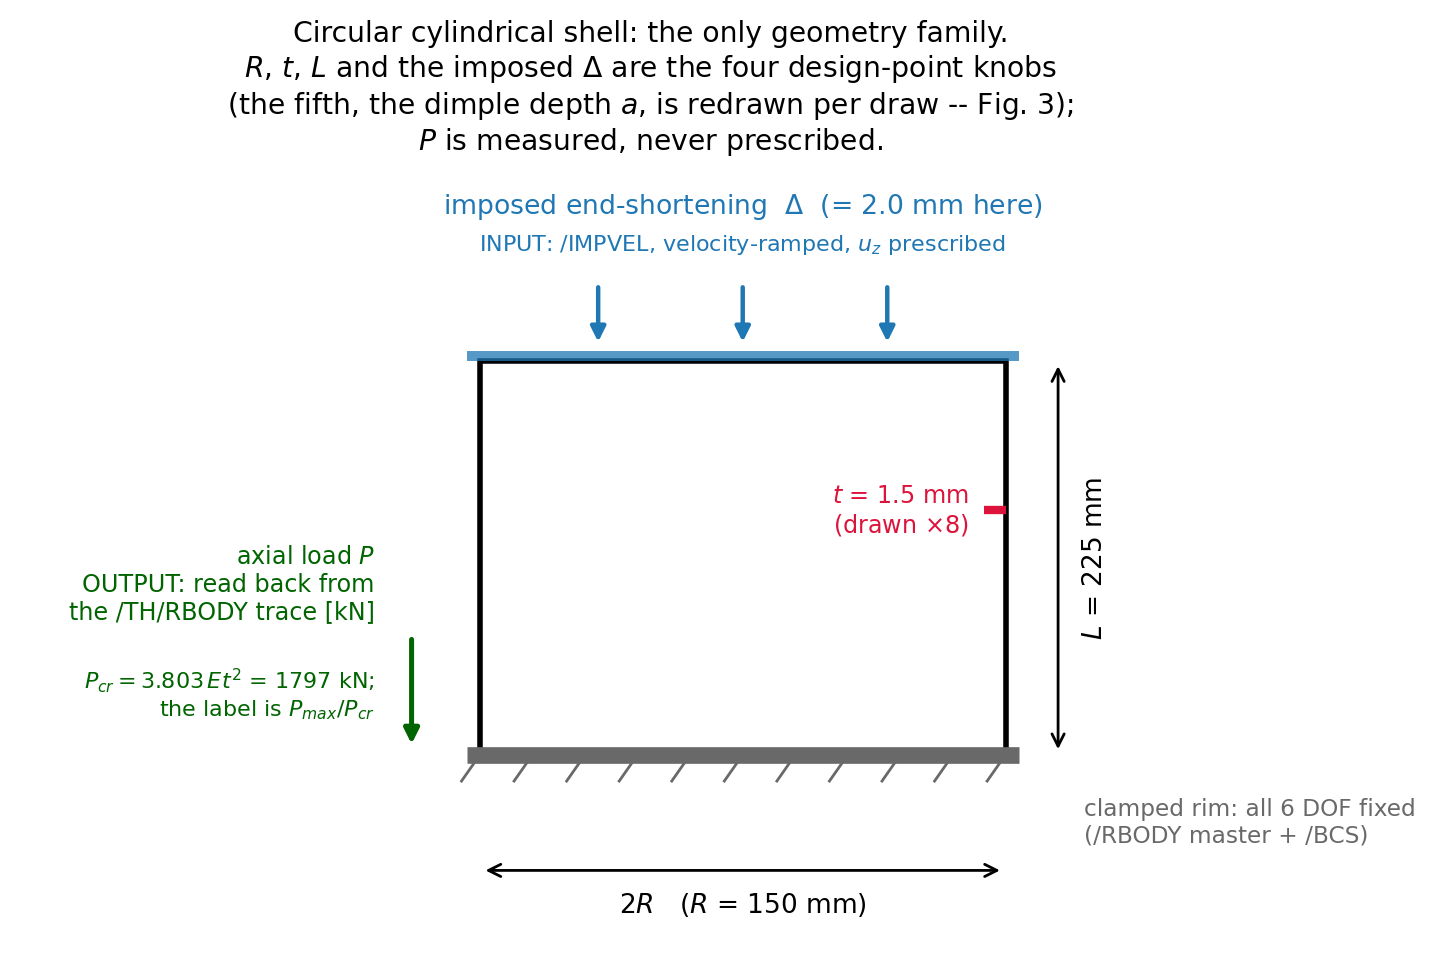
\includegraphics[width=0.92\linewidth]{figures/geometry_schematic.png}
\caption{해석 조건. 공칭 원통($R=150$, $t=1.5$(그림에서 8배 과장), $L=225$\,mm,
  설계 공간 중심)이다. 하단 테두리는 \code{/RBODY}+\code{/BCS}로 6자유도를
  구속한다. 상단 테두리에는 \code{/IMPVEL}로 축방향 변위 $\Delta$를 속도
  $v=0.25$\,mm/ms로 준다. 반력 $P$는 입력이 아니라 출력이며
  \code{/TH/RBODY}에서 읽는다. 고전 좌굴하중은 $P_{cr}=3.803\,E t^2$(중심에서
  1797\,kN)다.}
\label{fig:geom}
\end{figure}

\begin{figure}[!htbp]
\centering
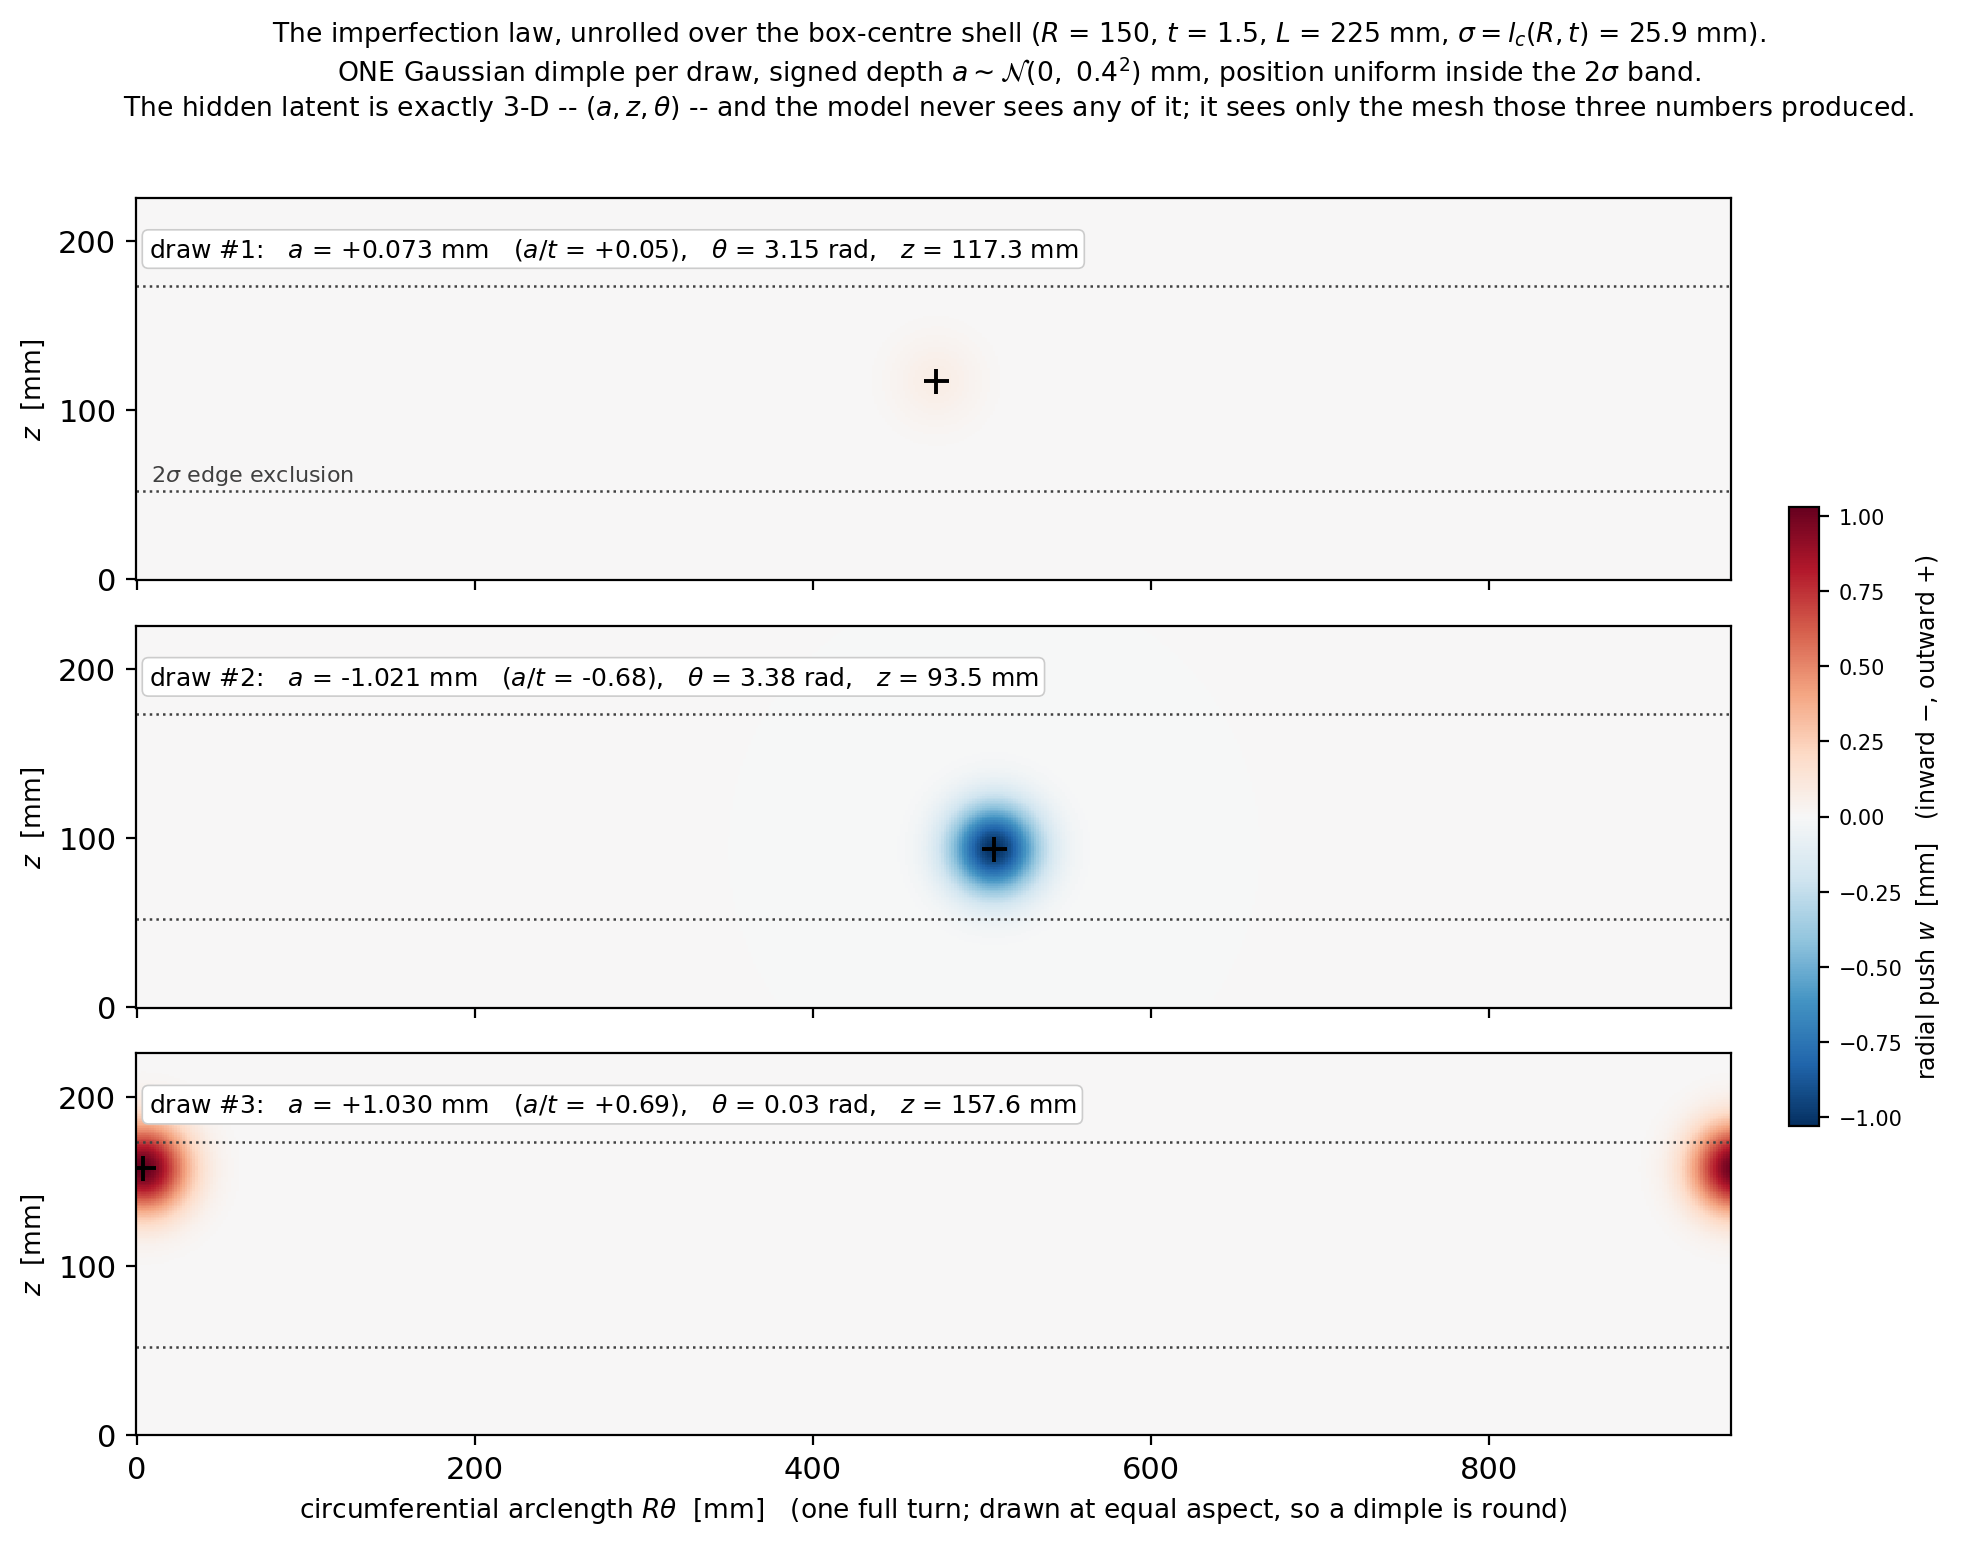
\includegraphics[width=\linewidth]{figures/imperfection_dimples.png}
\caption{숨은 결함 $\xi$. 중심 형상의 펼친 셸 위에 그린 세 표본이다
  ($a=+0.073$, $-1.021$, $+1.030$\,mm). 가우시안 딤플의 폭은 $\sigma=l_c$
  (중심에서 25.9\,mm)이고, 중심은 양 끝에서 $2\sigma$ 떨어진 영역(점선) 안에
  균일하게 놓인다. 결함은 솔버의 초기 형상에만 들어간다. \textbf{모델 입력은
  결함 없는 공칭 원통이다.}}
\label{fig:dimples}
\end{figure}

\begin{figure}[!htbp]
\centering
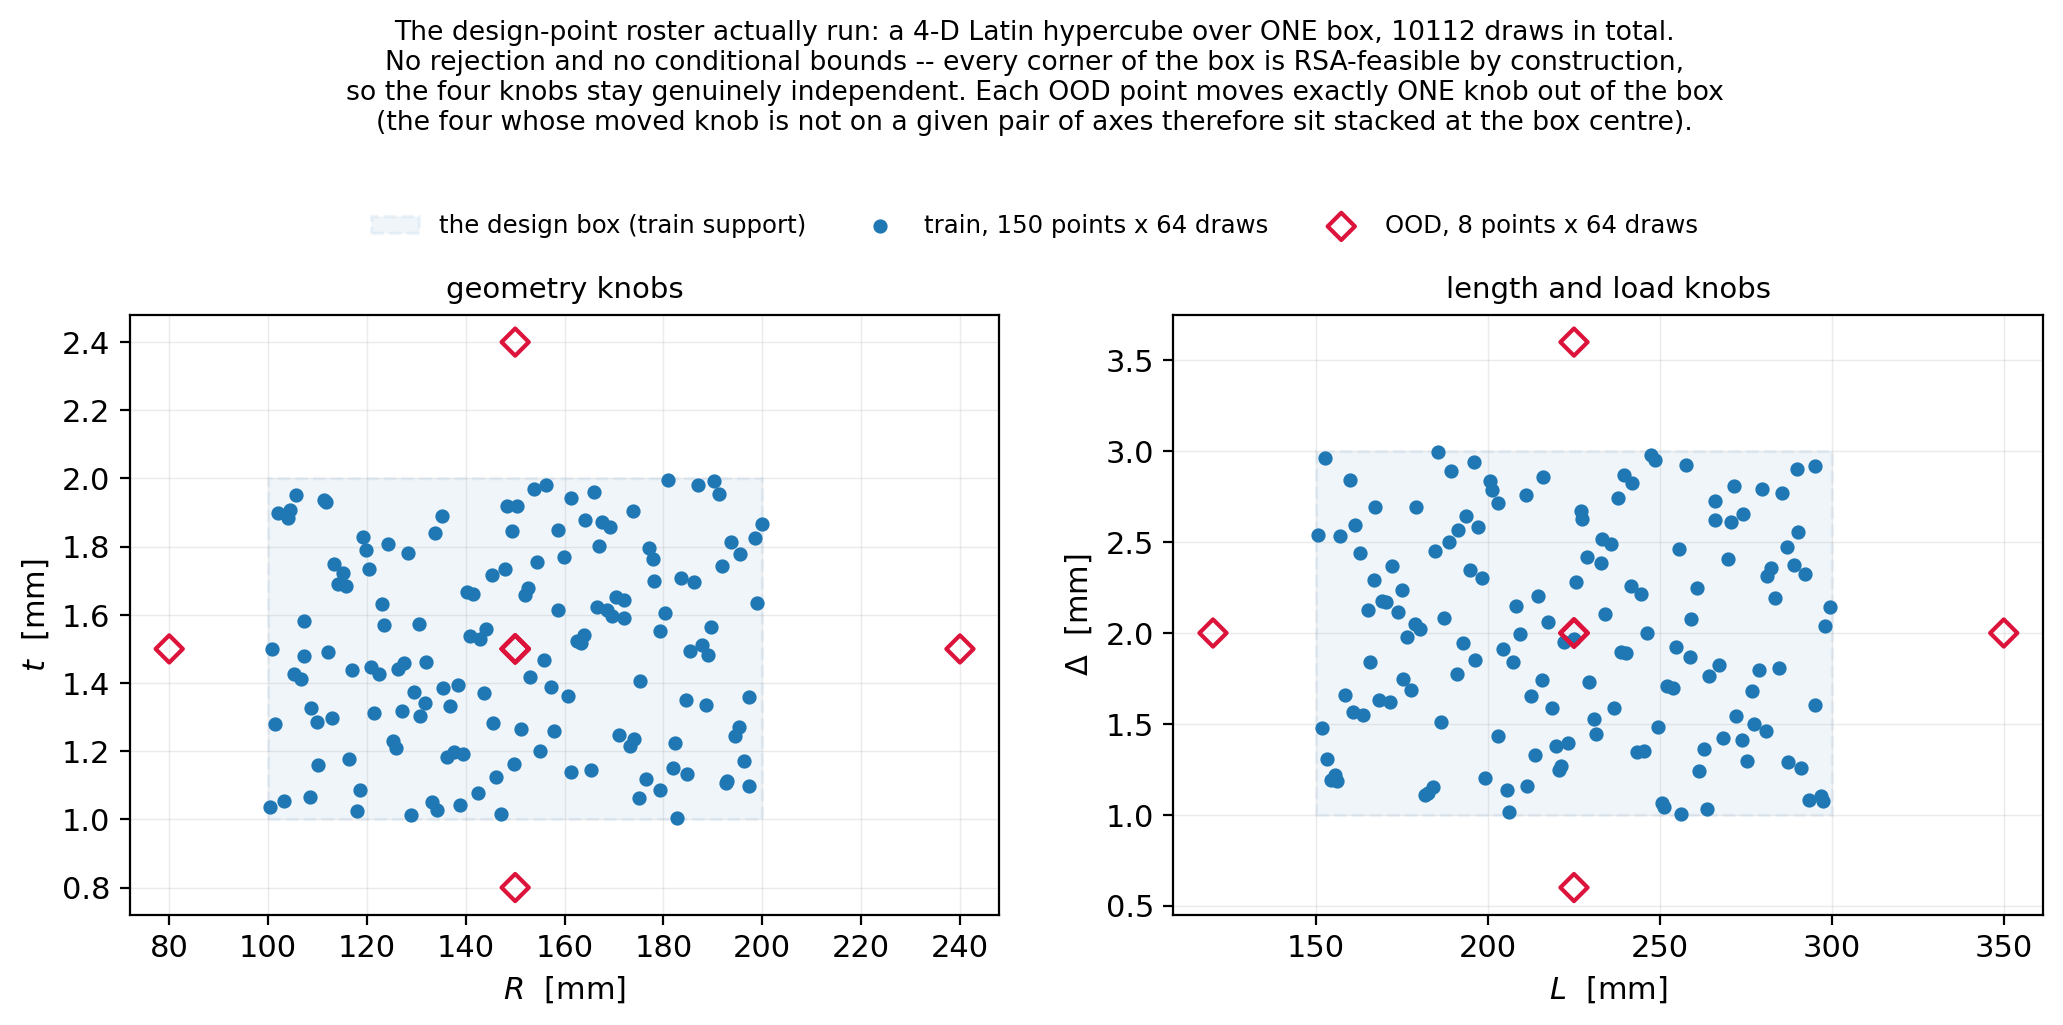
\includegraphics[width=0.95\linewidth]{figures/design_box.png}
\caption{생성 시점의 설계 공간. 학습 150 형상(4차원 LHS) $\times$ 64 표본과,
  중심에서 한 축만 옮긴 OOD 8 형상 $\times$ 64 표본, 모두 10,112 표본이다.
  평가 때 OOD는 형상당 200 표본으로 늘렸다(그림~\ref{fig:eval}).}
\label{fig:design}
\end{figure}

\begin{table}[!htbp]
\centering
\footnotesize
\begin{tabularx}{\textwidth}{@{}l Y@{}}
\toprule
항목 & 값 \\
\midrule
설계 변수 & $R\sim U[100,200]$, $t\sim U[1,2]$, $L\sim U[150,300]$, $\Delta\sim U[1,3]$ (mm); 4차원 LHS 150 형상 \\
결함 & 형상당 64 표본; $a\sim\N(0,0.4^2)$\,mm; $\sigma=l_c=\pi\sqrt{Rt}/[12(1-\nu^2)]^{1/4}$; 중심은 $2\sigma$ 끝단 배제 영역 안에서 균일, $\theta_c$ 균일 \\
재료 & 선형 탄성 강(\code{/MAT/ELAST}, 항복 없음), $E=210$\,GPa, $\nu=0.3$, $\rho=7.85\times10^{-6}$\,kg/mm$^3$ \\
요소·메시 & 정렬 사각 셸, QEPH, 두께 적분점 $N=5$; $h\le l_c/10$; 24,852--87,398 노드(중앙값 45,623) \\
솔버 & OpenRadioss explicit, 단위계 kg--mm--ms \\
경계 조건 & 하단 테두리 6자유도 구속; 상단 \code{/IMPVEL} $u_z$, $v=0.25$\,mm/ms(램프) \\
기준량 & $P_{cr}=3.803\,Et^2$; $d_{cr}=0.60523\,tL/R$; 하중비 $\lambda=\Delta/d_{cr}$ \\
HDF5 행 & 0:3 좌표, 3:6 변위 $u$, 6 두께 $t$, 7 강제변위 $\Delta$, 8 노드 타입; \code{input\_var 3}, \code{output\_var 3}, \code{cond\_var 2} \\
분할 & \code{split\_group\_attr shape\_idx}(형상 단위); test 15 형상 \\
OOD & 중심 $(150, 1.5, 225, 2.0)$에서 한 축만: $R$ 80/240, $t$ 0.8/2.4, $L$ 120/350, $\Delta$ 0.6/3.6 \\
\bottomrule
\end{tabularx}
\caption{원통 셸 좌굴(ex3) 데이터셋. 결함 $\xi=(a,z_c,\theta_c)$는 HDF5의
  \code{latent/} 그룹에 진단용으로만 저장되고, 입력 행에는 없다.}
\label{tab:dataset}
\end{table}

\subsection{모델 설정}

\begin{table}[!htbp]
\centering
\footnotesize
\begin{tabularx}{\textwidth}{@{}l Y@{}}
\toprule
공통 & DDP; batch 2 $\times$ accum 4; lr $10^{-4}$, wd $10^{-4}$, warmup 5; augment; AMP; checkpointing; EMA 0.99; \code{latent\_dim 128}; \code{voronoi\_seedmean} 4096/256; \code{mp\_per\_level 2,3,5,3,2}; \code{hierarchy\_variants 2}, \code{hierarchy\_seed 42}; \code{positional\_features 4}; \code{best\_by crps} \\
\midrule
HI-MGN-V & 120 epoch; \code{vae\_latent\_dim 32}($\times3$ 슬롯); \code{vae\_mp\_layers 3}; \code{graph\_aware}; \code{alpha\_recon 1000}; \code{lambda\_mmd 1}(median); \code{posterior\_min\_std 0.05}; \code{beta\_aux 10}; AdaLN; prior \code{gnn\_e2e} FM, \code{prior\_mp\_layers 3}, hidden 128, \code{prior\_nll\_weight 1}, \code{prior\_grad\_to\_encoder 0}; \code{prior\_fm\_steps 30} Heun; \code{prior\_freeze} 80 \\
cHI-MGNflow & \code{latent\_ch 4}; \code{ae\_kl\_weight 1e-6}; \code{ae\_epochs 60}, \code{training\_epochs 120}; \code{prior\_blocks 4}; \code{flow\_time\_freqs 16}; $t$ uniform, $w$ uniform; \code{flow\_steps 30} Heun; \code{predict sample}; \code{val\_flow\_steps 30}, \code{val\_num\_samples 8}; \code{prior\_global} 미지정(\code{none}) \\
\bottomrule
\end{tabularx}
\caption{ex3 baseline 설정
  (\code{configs/MeshGraphNets\_Variational/probabilistic/ex3/baseline/config\_train\_himgn\_v.txt},
  \code{configs/HI\_MGNFlow/probabilistic/ex3/baseline/config\_train\_chi\_mgnflow.txt}).
  \S\ref{sec:results}의 비교는 이 두 설정으로 학습한 모델이다.}
\label{tab:configs}
\end{table}

\subsection{평가 프로토콜}\label{sec:eval}

\begin{figure}[!htbp]
\centering
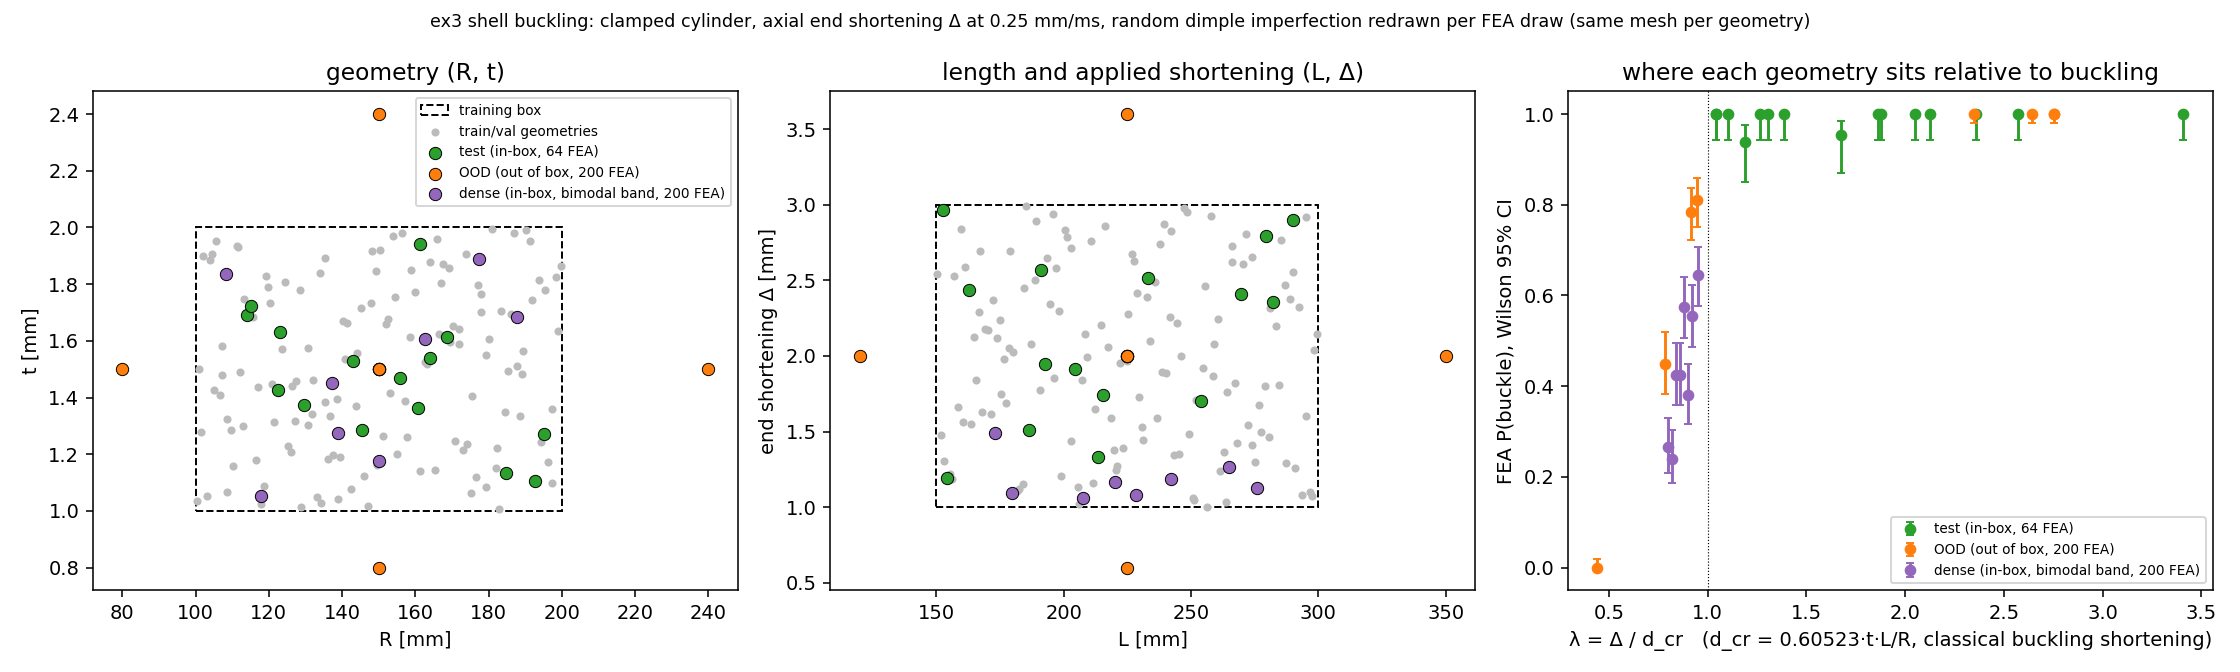
\includegraphics[width=\linewidth]{figures/eval_setup.png}
\caption{평가 집합.
  (i) test: 학습에 없던 15 형상 $\times$ FEA 64.
  (ii) OOD: 8 형상 $\times$ FEA 200.
  (iii) dense: 상자 안이지만 전이 구간 $\lambda=0.80$--0.95에 놓인 8 형상
  $\times$ FEA 200.
  $(R,t)$, $(L,\Delta)$ 평면의 위치와 FEA 좌굴 확률(Wilson 95\% 구간)을
  함께 보였다.}
\label{fig:eval}
\end{figure}

\paragraph{통계량.} 표본마다 최대 노드 변위 크기 $s=\max_i\|u_i\|$를 쓴다.
좌굴 판정 문턱은 5.17\,mm다. 이 문턱은 비좌굴 표본의 최댓값과 좌굴 표본의
최솟값 사이에서 정했으며, 솔버의 좌굴 플래그와 4159 표본 중 97.5\%에서
일치한다(OOD 표본 하나는 시간 초과로 빠졌다).

\paragraph{지표.} 형상마다 모델 표본 1000개와 FEA 표본을 비교한 뒤, 집합별로
평균한다. 아래에서 $\mathrm{sd}_{\text{FEA}}$는 FEA 표본의 표준편차다.
\begin{itemize}
\item 평균비: $\overline{s}_{\text{model}}/\overline{s}_{\text{FEA}}$.
\item sd비: $\mathrm{sd}_{\text{model}}/\mathrm{sd}_{\text{FEA}}$.
\item W1/sd: $W_1/\mathrm{sd}_{\text{FEA}}$.
\item CRPS/sd: FEA 표본마다 모델 앙상블의 CRPS를 계산해 평균한 뒤
  $\mathrm{sd}_{\text{FEA}}$로 나눈다.
\item KS: 두 경험분포 사이의 KS 통계량.
\item $|\Delta P|$: $|P_{\text{model}}(\text{buckle})-P_{\text{FEA}}(\text{buckle})|$.
\end{itemize}
\paragraph{노이즈 바닥.} FEA 표본 수가 유한하므로 완벽한 모델도 0을 얻지
못한다. 바닥은 FEA 표본을 반으로 나눠 서로 비교해 구한다. W1/sd 바닥은
FEA 표본 수에 따라 다음과 같다(평균 / 90분위).
\begin{center}
\begin{tabular}{@{}lcccc@{}}
\toprule
FEA 표본 수 & 16 & 32 & 64 & 100 \\
W1/sd & 0.263 / 0.455 & 0.189 / 0.329 & 0.151 / 0.265 & 0.144 / 0.245 \\
\bottomrule
\end{tabular}
\end{center}
완벽한 모델의 CRPS/sd는 약 0.52--0.54다.

\subsection{결과}\label{sec:results}

\begin{table}[!htbp]
\centering
\small
\begin{tabular}{@{}llcccccc@{}}
\toprule
집합 & 모델 & 평균비 & sd비 & W1/sd & CRPS/sd & KS & $|\Delta P|$ \\
\midrule
test (15$\times$64) & cHI-MGNflow & \textbf{1.018} & 0.664 & \textbf{0.692} & \textbf{0.756} & \textbf{0.389} & \textbf{0.005} \\
 & HI-MGN-V & 0.832 & 1.251 & 1.375 & 1.003 & 0.541 & 0.087 \\
 & \textit{바닥} & & & 0.290 & 0.538 & 0.213 & \\
\midrule
OOD (8$\times$200) & cHI-MGNflow & \textbf{1.068} & 0.486 & \textbf{0.829} & \textbf{0.838} & \textbf{0.500} & \textbf{0.100} \\
 & HI-MGN-V & 0.795 & 1.064 & 1.630 & 1.370 & 0.698 & 0.158 \\
 & \textit{바닥} & & & 0.141 & 0.511 & 0.104 & \\
\midrule
dense (8$\times$200) & cHI-MGNflow & 1.122 & 0.531 & \textbf{0.501} & \textbf{0.649} & \textbf{0.418} & \textbf{0.100} \\
 & HI-MGN-V & 0.627 & 0.659 & 0.557 & 0.666 & 0.425 & 0.276 \\
 & \textit{바닥} & & & 0.112 & 0.524 & 0.096 & \\
\bottomrule
\end{tabular}
\caption{최대 변위 $s=\max_i\|u_i\|$의 형상별 분포 비교(모델 표본 1000/형상,
  집합 평균). 평균비와 sd비의 목표는 1이고, 나머지는 바닥에 가까울수록 좋다.
  형상별 값은 부록~\ref{app:pergeom}에 있다.}
\label{tab:results}
\end{table}

\begin{figure}[!htbp]
\centering
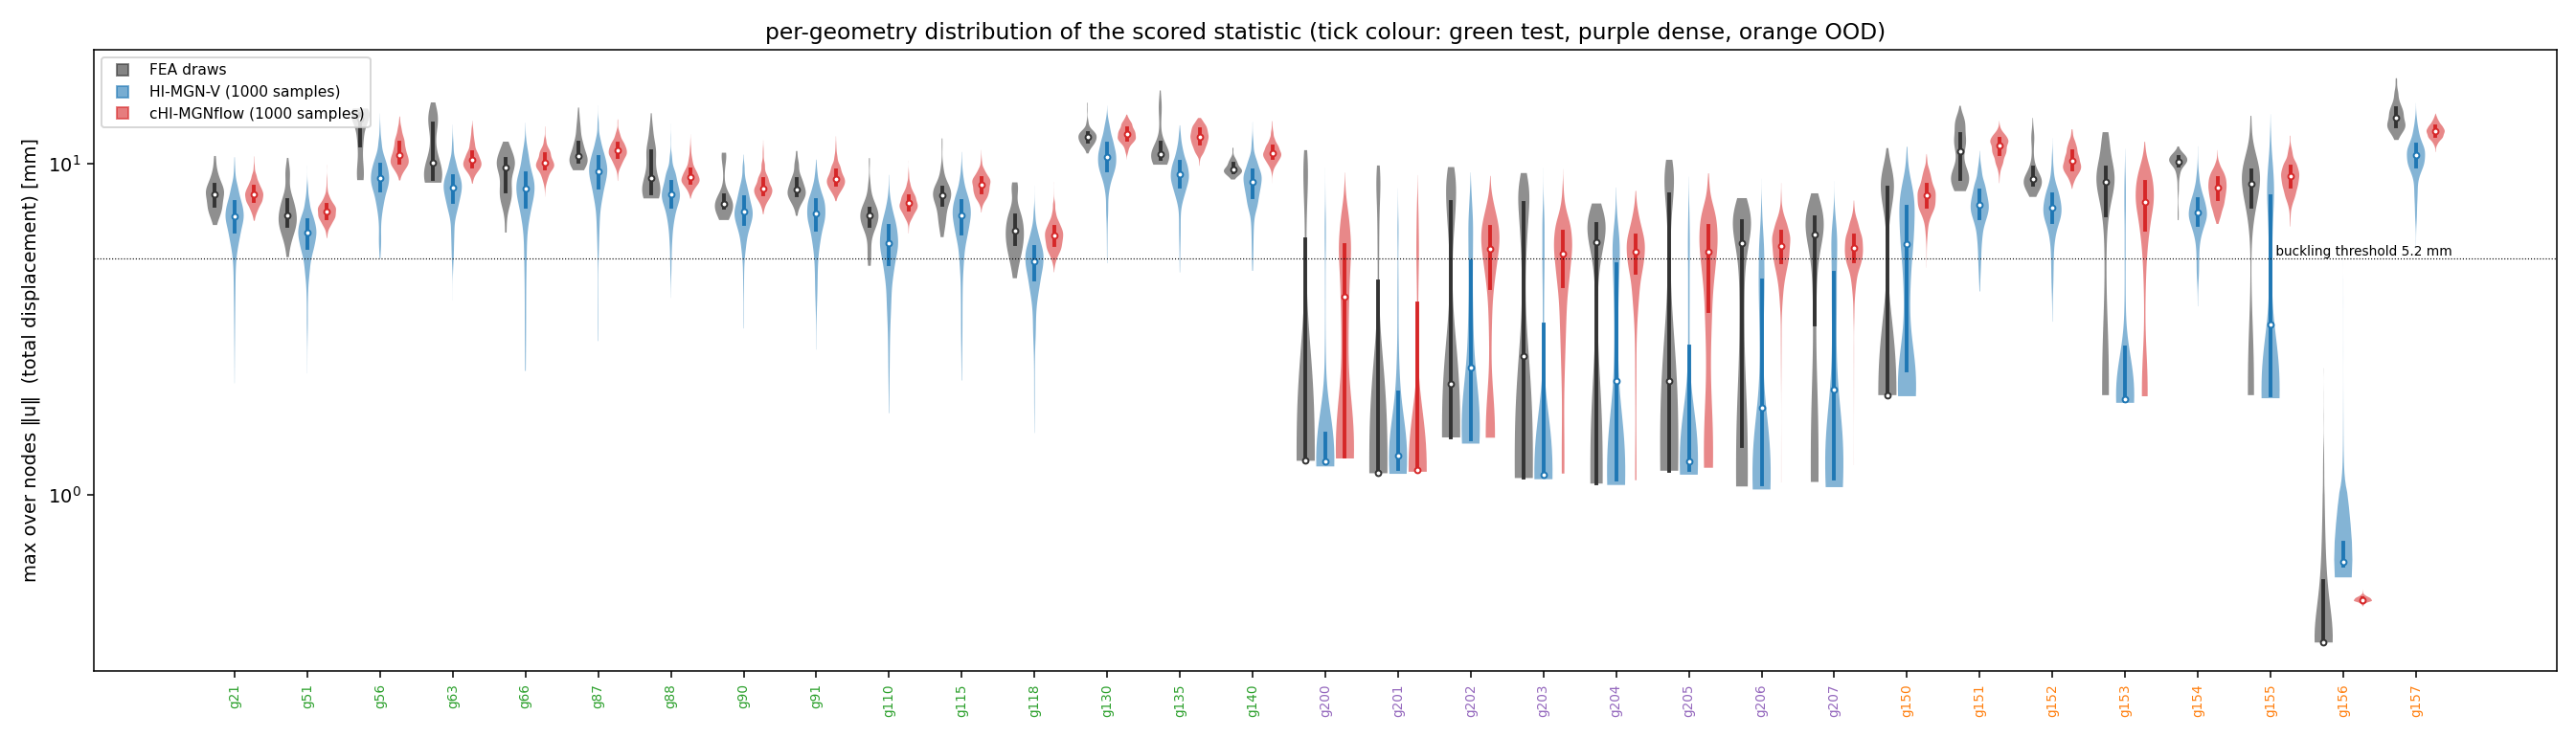
\includegraphics[width=\linewidth]{figures/dense_violins.png}
\caption{형상별 최대 변위 분포(로그 축). FEA, HI-MGN-V(1000 표본),
  cHI-MGNflow(1000 표본)이고, 점선은 좌굴 문턱 5.2\,mm다. cHI-MGNflow는
  중심은 맞지만 폭이 좁다. HI-MGN-V는 전체가 아래로 밀려 있고, 큰 분기에
  가야 할 질량이 아래 꼬리에 남는다.}
\label{fig:violins}
\end{figure}

\begin{figure}[!htbp]
\centering
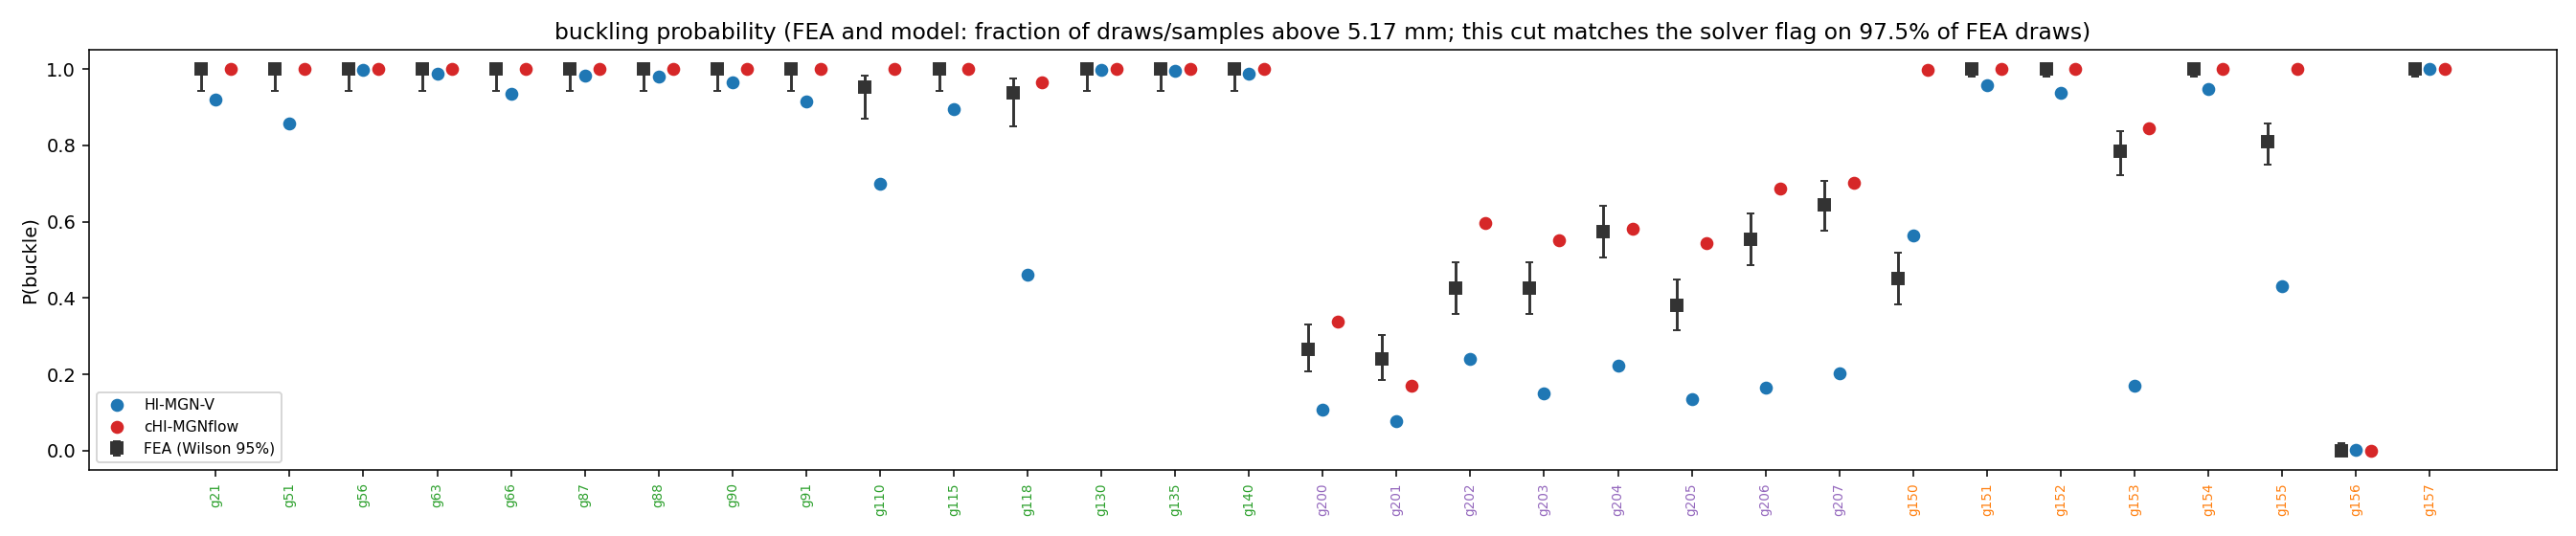
\includegraphics[width=\linewidth]{figures/dense_pbuckle.png}
\caption{형상별 좌굴 확률. FEA는 Wilson 95\% 구간과 함께 보였다. 문턱
  5.17\,mm는 솔버 플래그와 97.5\% 일치한다.}
\label{fig:pbuckle}
\end{figure}

\begin{figure}[!htbp]
\centering
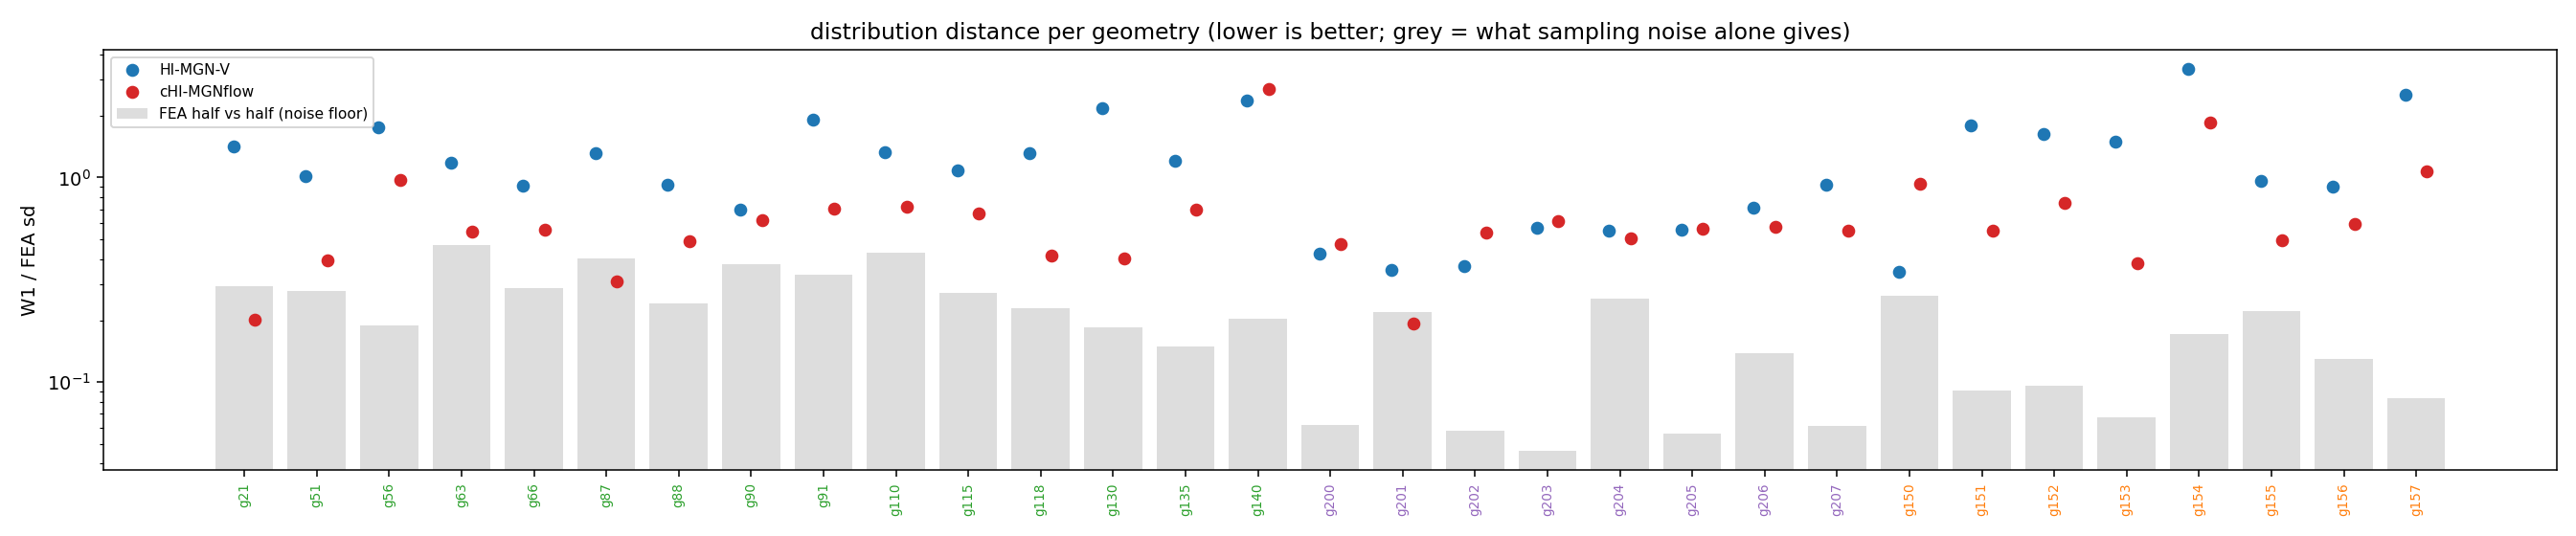
\includegraphics[width=\linewidth]{figures/dense_w1.png}
\caption{형상별 W1/sd. 회색은 FEA 반-대-반 노이즈 바닥이다.}
\label{fig:w1}
\end{figure}

\paragraph{관찰.}
\begin{enumerate}
\item \textbf{test와 OOD에서는 cHI-MGNflow가 분명히 낫다.} test W1/sd는 0.69 대
  1.38이고, OOD CRPS/sd는 0.84 대 1.37이다. 두 모델이 틀리는 방식은 다르다.
  \begin{itemize}
  \item cHI-MGNflow는 평균이 맞고(1.02) 폭이 좁다. sd비는 평균 0.66이고 중앙값은
    0.58이다. g140의 1.65가 평균을 끌어올렸다.
  \item HI-MGN-V는 평균이 0.83배로 작다. sd비가 1을 넘는 것(1.25)은 폭이 맞아서가
    아니다. 잘못된 분기 쪽으로 긴 아래 꼬리가 생겨서다(그림~\ref{fig:violins}).
  \end{itemize}
\item \textbf{좌굴 확률.} cHI-MGNflow는 좌굴을 과대 예측한다. 예를 들어 g150은
  1.00 대 FEA 0.45이고, g155는 1.00 대 0.81이다. HI-MGN-V는 dense 구간에서
  과소 예측한다(0.08--0.24 대 FEA 0.24--0.65).
\item \textbf{dense 구간에서는 거의 비긴다.} W1/sd는 0.50 대 0.56, CRPS/sd는
  0.65 대 0.67, KS는 0.42 대 0.42다. 차이는 $|\Delta P|$(0.10 대 0.28)와 평균비
  (1.12 대 0.63)에 있다.
\item 이전 평가도 같은 방향이다. OOD 8 형상 $\times$ 64, 통계량 $u_x$ 범위로
  비교한 결과는 다음과 같다.
  \begin{center}
  \small
  \begin{tabular}{@{}lccccc@{}}
  \toprule
  & CRPS/sd & 평균 편차/sd & sd비 & PIT KS & W1/sd \\
  \midrule
  cHI-MGNflow & 0.360 & $-0.01$ & 0.81 & 0.28 & 0.22 \\
  HI-MGN-V & 0.664 & $-0.69$ & 0.71 & 0.62 & 0.69 \\
  \bottomrule
  \end{tabular}
  \end{center}
  HI-MGN-V 표본에 test split에서 맞춘 단일 배율 $\alpha=1.45$를 곱하면 OOD
  CRPS/sd가 0.385, W1/sd가 0.31로 내려간다. 즉 HI-MGN-V 오차의 상당 부분은
  전체 진폭의 축소다.
\end{enumerate}

\subsection{HI-MGN-V 진단: 인코더가 병목이다}\label{sec:diag-v}

\paragraph{전체 모델.}
\begin{itemize}
\item 학습 표본을 posterior 평균으로 디코딩하면 진폭이 FEA의 0.72배다
  (중앙값, 범위 0.56--0.81).
\item 설명 비율은 $1-\text{재구성 MSE}/\text{$z$ 없는 바닥 MSE}$로 정의한다.
  바닥은 형상별 표본 평균 필드로 예측했을 때의 MSE다.
\item 검증 재구성 0.287, 바닥 0.540이므로 $z$는 표본 간 변동의 약 47\%만
  설명한다. 바닥은 train 0.529, val 0.540, test 0.683이다.
\end{itemize}

\paragraph{20 형상 부분실험.} 그림~\ref{fig:diag-setup}(c)의 20개 형상으로
세 arm을 비교했다.
\begin{itemize}
\item 분할은 16/2/2, batch 1 $\times$ accum 8, 100 epoch, \code{prior\_freeze 0}이다.
\item 배치 1이라 MMD는 상수다. VRAM은 batch 1 기준이다.
\item 바닥은 train 0.535, valid 1.012, test 0.475다.
\end{itemize}
\begin{center}
\small
\begin{tabular}{@{}lccccc@{}}
\toprule
arm & train 재구성 & valid 재구성 & CRPS & 바닥 탈출 epoch & VRAM \\
\midrule
base (\code{vae\_mp\_layers 3}, $z$ 32) & 0.529 & 1.138 & 0.615 & 탈출 못 함 & 10.3\,GB \\
mp8 (8, 32) & 0.288 & 0.854 & 0.529 & 35 & 14.2\,GB \\
mp8z128 (8, 128) & 0.286 & 0.850 & 0.541 & 35 & --- \\
\bottomrule
\end{tabular}
\end{center}
인코더 깊이를 3에서 8로 늘려야만 재구성이 바닥 아래로 내려간다. 잠재 크기를
32에서 128로 늘리는 것은 효과가 없다. 즉 병목은 잠재 용량이 아니라 인코더의
수용영역이다.

\begin{figure}[!htbp]
\centering
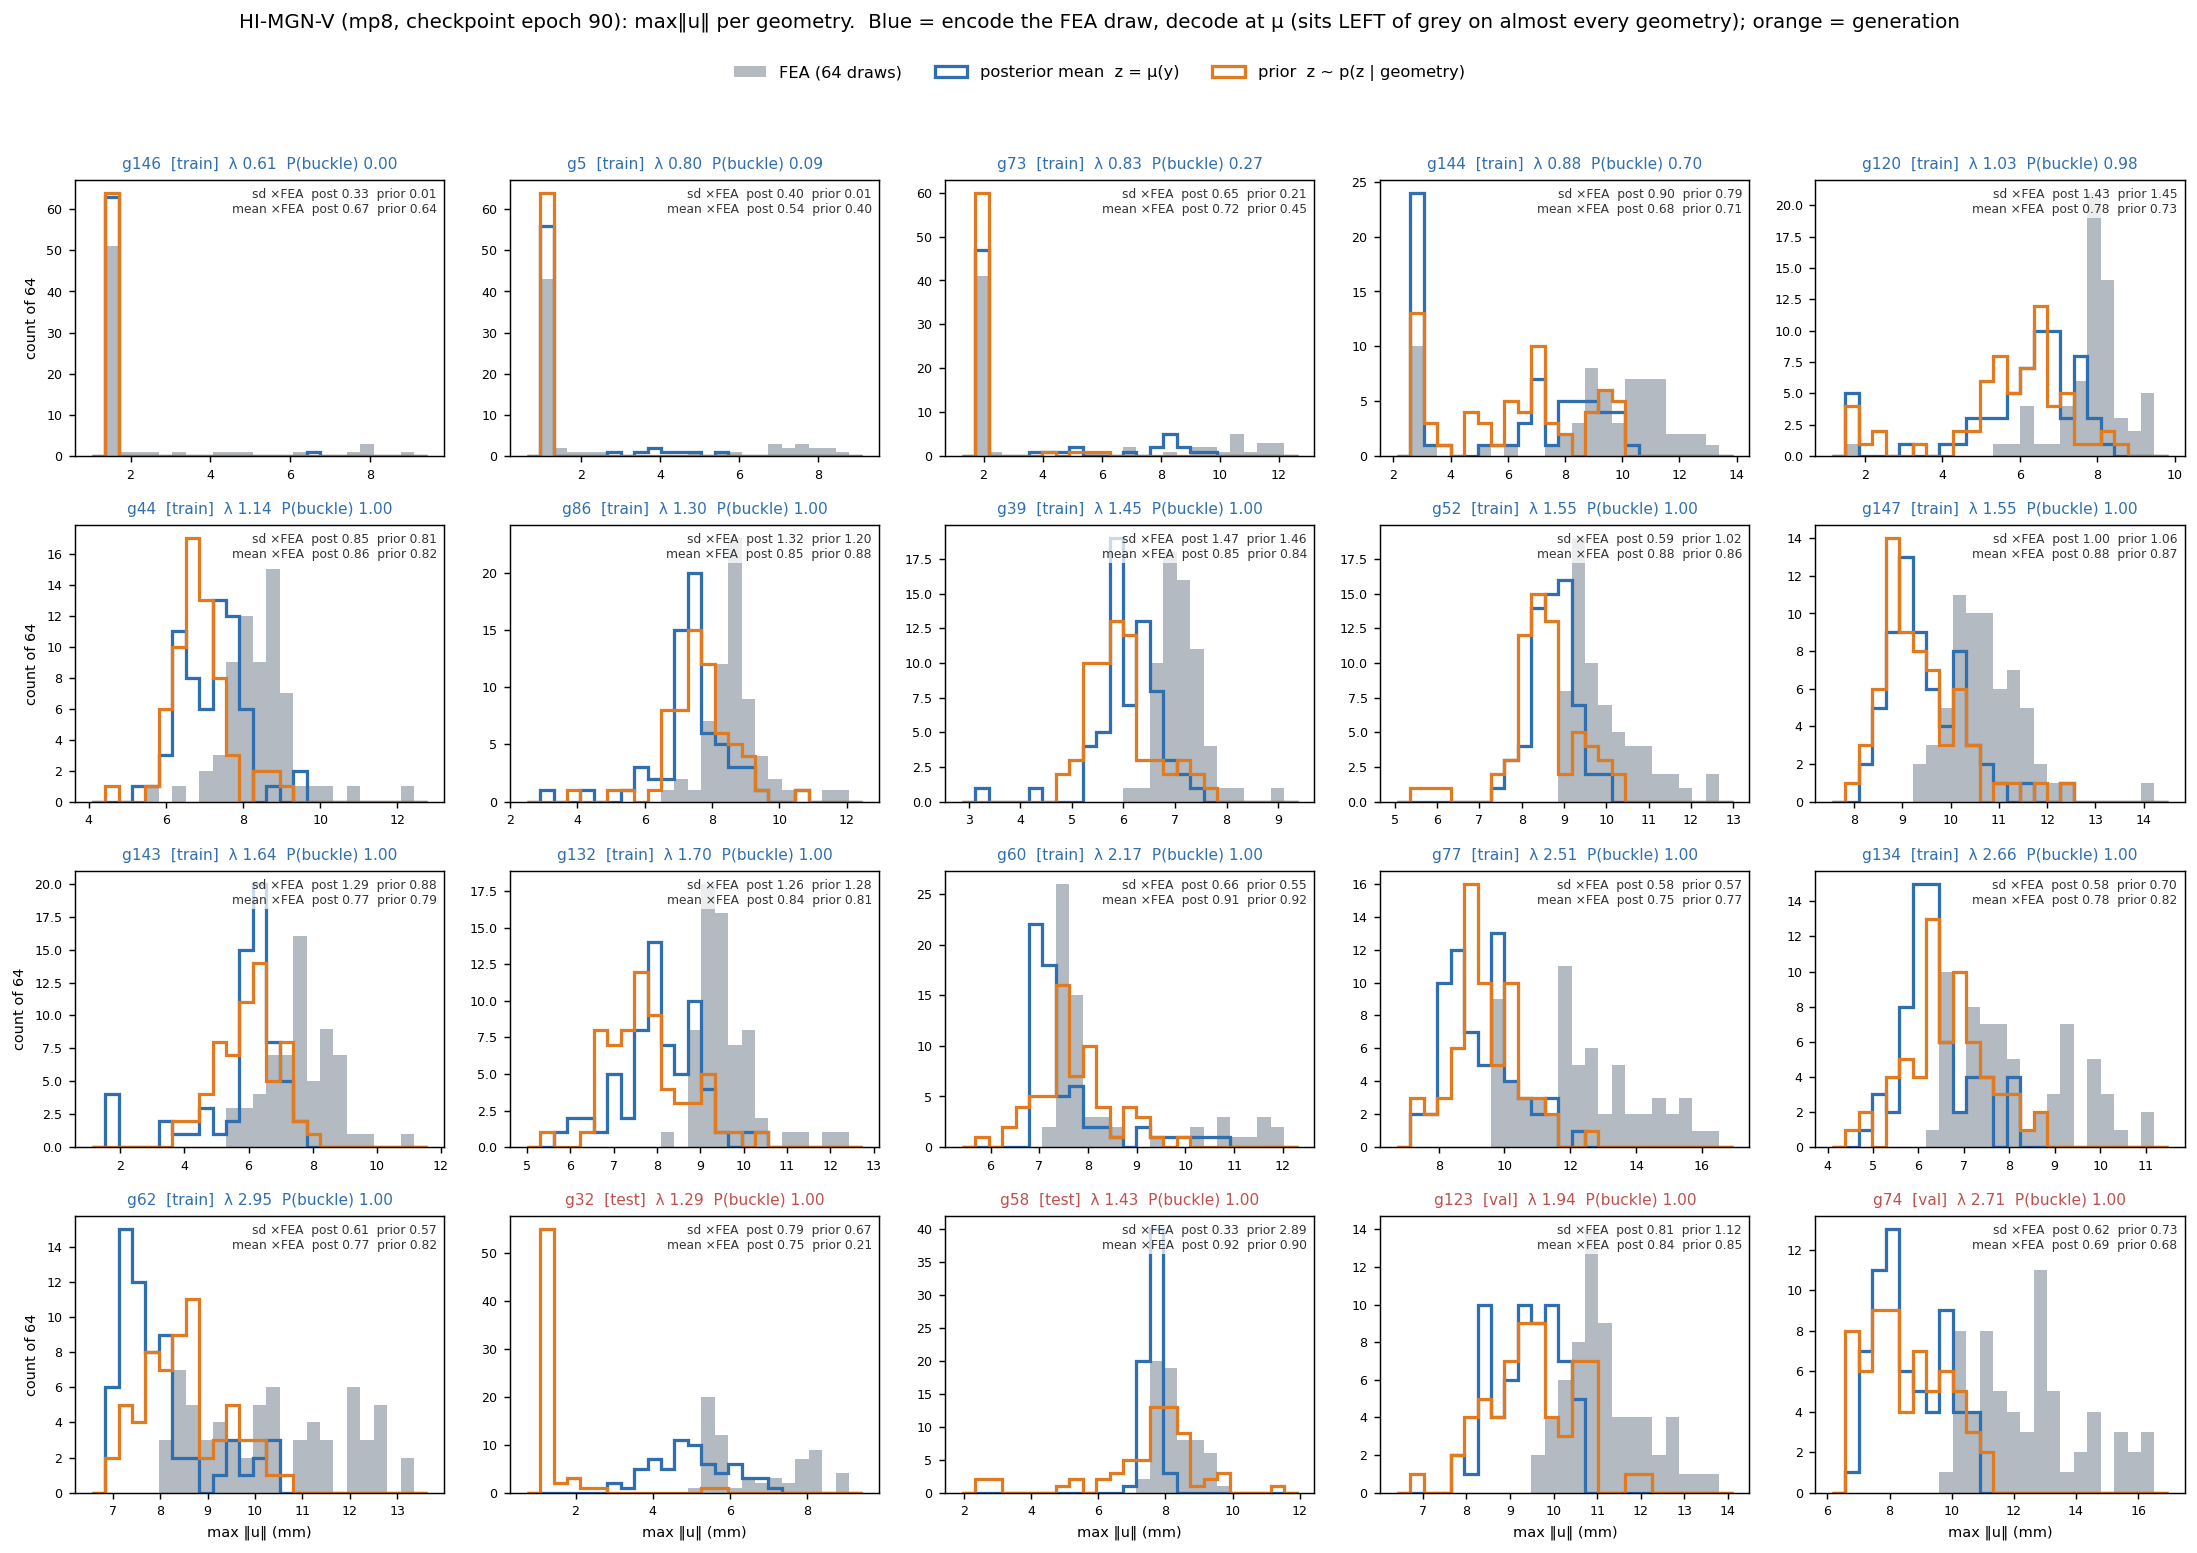
\includegraphics[width=\linewidth]{figures/himgnv_mp8_hist.png}
\caption{mp8 arm, epoch 90의 20 형상 히스토그램. 회색은 FEA, 파랑은 posterior
  평균 디코딩, 주황은 prior 표본이다. 각 패널에 sd비와 평균비를 적었다.}
\label{fig:mp8}
\end{figure}

mp8의 epoch 90 지표(train 16 / held 4 형상)는 다음과 같다.
\begin{itemize}
\item posterior 평균 진폭: 0.78 / 0.80.
\item posterior sd비: 0.75 / 0.70.
\item 형상 내 기울기(디코딩 통계량 대 참값): 0.40 / 0.23.
\item 설명 비율: 0.41 / 0.01.
\end{itemize}
양봉 학습 형상(g5, g73, g144, g146)에서는 큰 분기 표본 100개 중 39개가 작은
분기로 디코딩된다. 맞는 분기로 간 표본의 진폭은 0.84배다. prior는 대체로
posterior와 비슷하다. 예외로 g146과 g5에서는 붕괴한다(sd 0.01). g32에서는 prior
표본 64개 중 55개가 잘못된 분기로 간다. base arm의 설명 비율은 0.01 / $-0.10$,
진폭은 0.35 / 0.31이다.

\begin{figure}[!htbp]
\centering
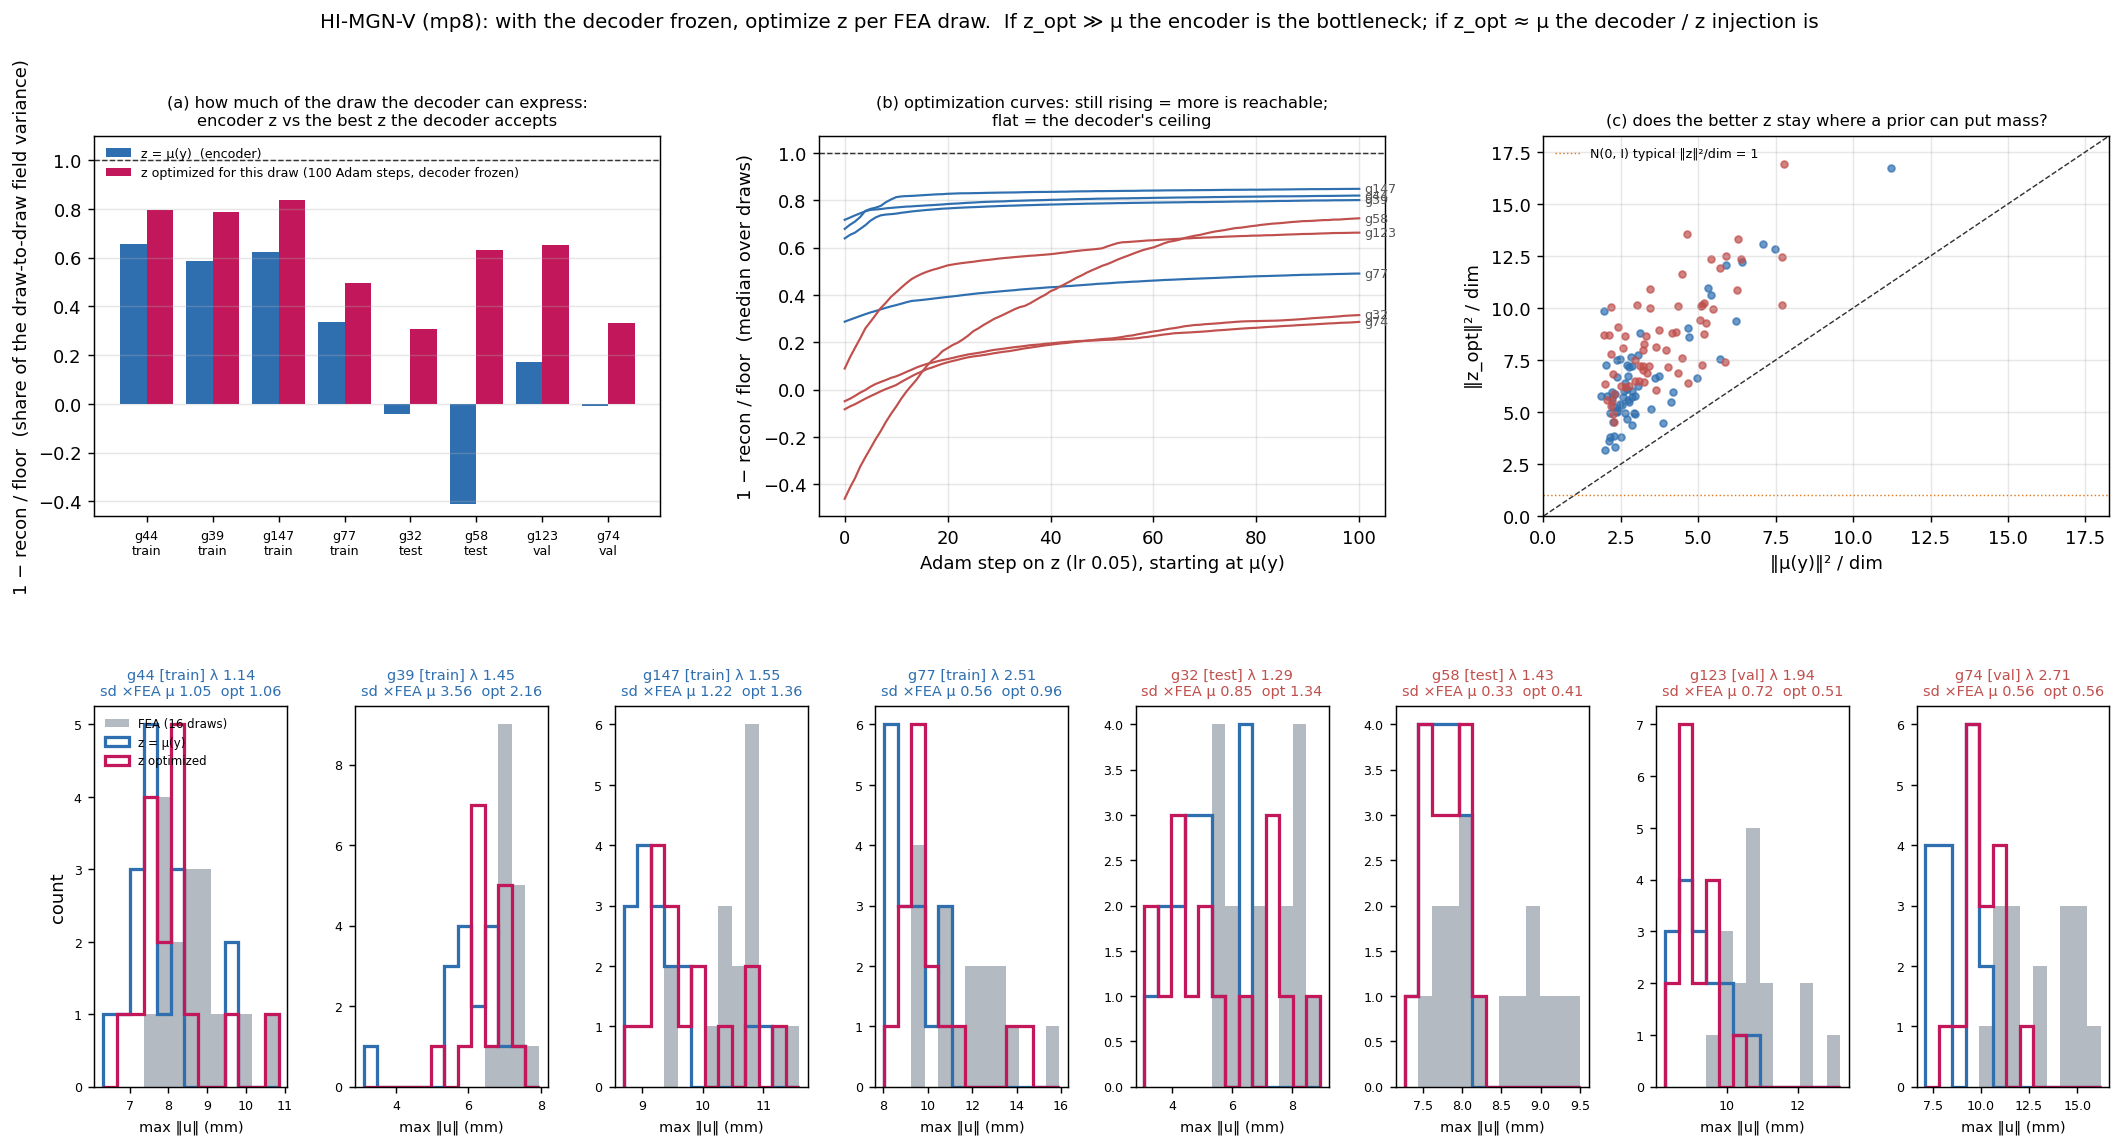
\includegraphics[width=\linewidth]{figures/himgnv_zopt.png}
\caption{같은 디코더에서 $z$를 직접 최적화한 결과(형상 8개, Adam 100 스텝,
  lr 0.05). (a) posterior 평균 $\mu$와 최적화된 $z_{\text{opt}}$의 설명 비율.
  (b) Adam 곡선. 100 스텝에서 평탄하다. (c) $\|z_{\text{opt}}\|^2/\dim$ 대
  $\|\mu\|^2/\dim$. 아래 줄은 FEA 16 표본과 비교한 히스토그램이다.}
\label{fig:zopt}
\end{figure}

\paragraph{$z$ 최적화.} 디코더를 고정하고 표본마다 $z$를 직접 최적화했다.
\begin{center}
\small
\begin{tabular}{@{}lcc@{}}
\toprule
 & 설명 비율 $\mu\to z_{\text{opt}}$ & 진폭 $\mu\to z_{\text{opt}}$ \\
\midrule
train & 0.34--0.66 $\to$ 0.49--0.84 & 0.78--0.90 $\to$ 0.87--0.94 \\
held & $-0.41$--0.17 $\to$ 0.31--0.65 & 0.67--0.92 $\to$ 0.77--0.93 \\
\bottomrule
\end{tabular}
\end{center}
$\|z_{\text{opt}}\|^2/\dim$은 $\|\mu\|^2/\dim$의 약 2배다. 이 결과에서 세 가지를
읽을 수 있다.
\begin{enumerate}
\item 같은 디코더로 훨씬 더 설명할 수 있으므로, \textbf{주 병목은 인코더}다.
\item 최적화해도 설명 비율은 0.85 이하에 머문다. 공간적으로 균일한 전역
  주입에는 표현력 상한이 있다.
\item $z_{\text{opt}}$는 posterior 구름 밖에 있다. 따라서 이 차이를 prior만
  개선해서 메울 수는 없다.
\end{enumerate}

\subsection{cHI-MGNflow 진단: prior가 노드 간 결합을 잃는다}\label{sec:diag-chi}

\paragraph{설정.} 동결된 AE 위에서 \code{train\_prior}로 \code{prior\_blocks 16}
prior를 학습했다. 형상 24개(train 9 / test 15)에 FEA 각 32 표본이다. 네 가지
잠재를 같은 디코더로 디코딩한다. $\mu_r$은 FEA 표본 $r$의 posterior 평균이다.
\begin{itemize}
\item posterior 평균: $\mu_r$.
\item prior: flow ODE로 얻은 $z_1'$.
\item shuffle: coarse 노드마다 독립적으로 고른 표본 $r_i$의 $\mu_{r_i,i}$.
  노드별 주변분포는 posterior와 같고 노드 간 결합은 없다.
\item coherent: $\bar\mu + \sum_r w_r(\mu_r-\bar\mu)$, $w\sim\N(0,1/(R-1))$.
  posterior의 노드 간 전체 공분산을 가진 가우시안이다. 정답 표본이 필요한
  오라클이다.
\end{itemize}

\begin{figure}[!htbp]
\centering
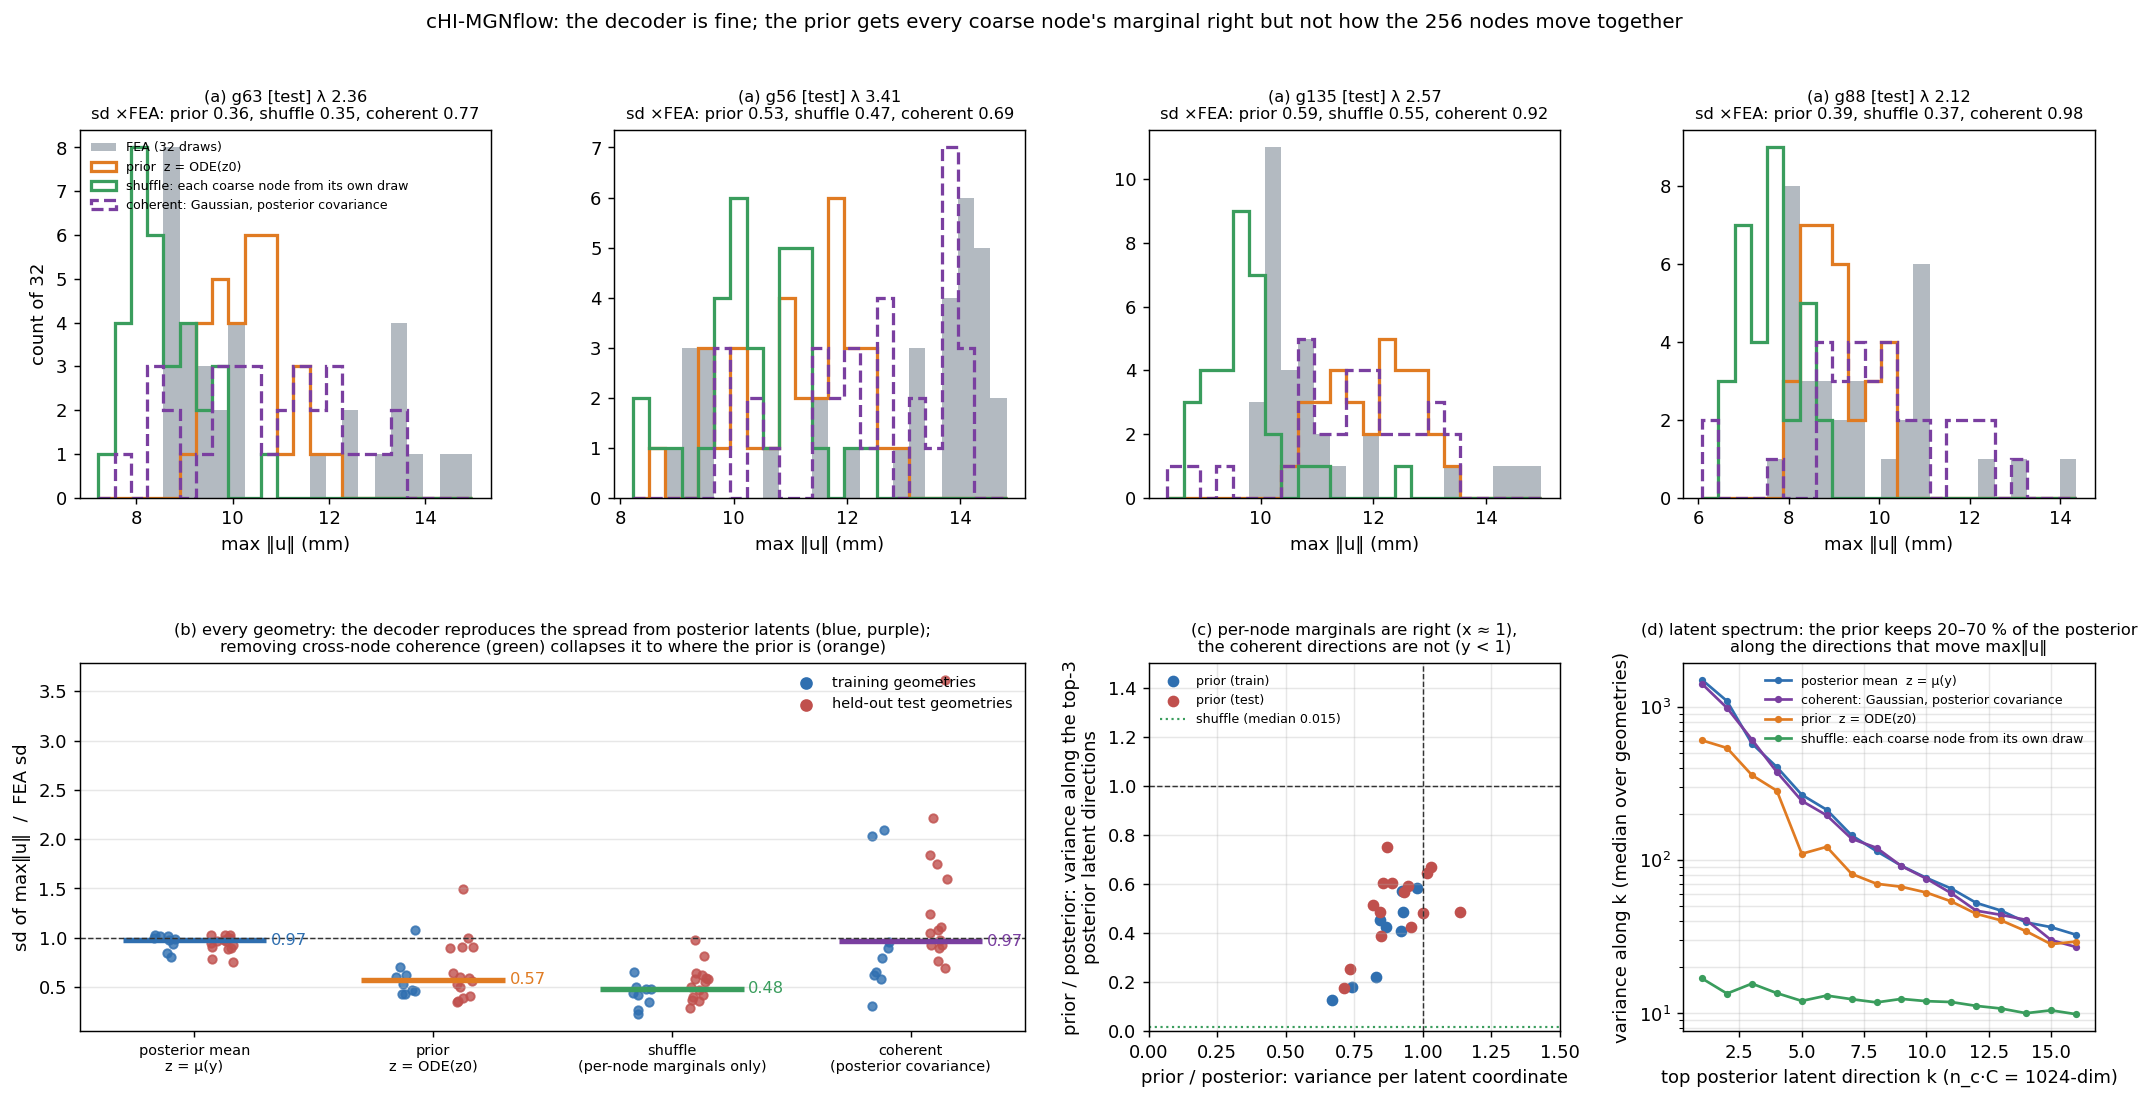
\includegraphics[width=\linewidth]{figures/chi_mechanism.png}
\caption{cHI-MGNflow 진단.
  (a) g63, g56, g135, g88의 히스토그램(FEA 32). prior, shuffle, coherent를
  비교했다.
  (b) sd비 중앙값. posterior 평균 0.97, prior 0.57, shuffle 0.48, coherent 0.97.
  (c) 좌표별 분산비는 약 1이지만, 상위 3개 주성분 방향의 분산비는 1보다
  작다(shuffle 중앙값 0.015).
  (d) 잠재 스펙트럼. prior는 상위 방향에서 posterior 분산의 20--70\%만 갖는다.}
\label{fig:chi-mech}
\end{figure}

\begin{center}
\small
\begin{tabular}{@{}lcccc@{}}
\toprule
sd비 & posterior 평균 & prior & shuffle & coherent \\
\midrule
train & 0.99 & 0.53 & 0.44 & 0.79 \\
test & 0.97 & 0.59 & 0.55 & 1.08 \\
\bottomrule
\end{tabular}
\end{center}
\begin{itemize}
\item posterior 평균비는 1.00이다. 즉 오토인코더는 정확하다.
\item prior 잠재의 좌표별 분산비는 0.86 / 0.89로 거의 맞다. 상위 3개 주성분
  방향의 분산비는 0.42 / 0.51에 그친다.
\item prior는 shuffle과 비슷하고, coherent는 FEA와 비슷하다. 따라서 디코더는
  정상이다. 실패는 prior가 \textbf{노드 사이의 결합}을 재현하지 못하는 데 있다.
  노드마다는 그럴듯하지만 서로 맞지 않는 잠재가 나오고, 디코더는 이를 두 분기
  사이의 필드로 만든다.
\item 블록을 4에서 16으로 늘린 효과는 작다. sd비 기하평균이 train 0.49
  $\to$ 0.55, test 0.59 $\to$ 0.62이고, 검증 CRPS는 둘 다 0.281이다.
\item flow 스텝을 30에서 100으로 늘려도 결과가 같다. 검증 CRPS는 prior epoch
  10부터 약 0.28에서 정체한다.
\end{itemize}
수용영역을 넓혀도 4 hop에서 16 hop으로 늘어날 뿐이다. 이 진단이
\S\ref{sec:token}의 전역 토큰을 추가한 직접적인 근거다. 원래 test split에서
측정한 값(prior sd비 중앙값 0.77, 범위 0.39--1.23)도 같은 방향이다.

\subsection{두 번째 데이터: SAOI 휨}\label{sec:saoi}

사내 SAOI 보드 휨(warpage) 데이터는 평가 집합 하나가 부품 하나의 공정 실현
125개다. 따라서 sd비의 목표는 1이다. 통계량은 $z$ 변위의 peak-to-valley다.

\paragraph{2026-09 비교} (각 모델 8-arm $2^{4-1}$ 스윕, 1000 epoch).
\begin{itemize}
\item MGN-V가 최고 W1/sd 0.410으로, cHI-MGNflow의 0.896보다 2.2배 낫다.
  MGN-V arm 2가 GPU 고장으로 빠져 있다는 점은 감안해야 한다.
\item 두 모델 모두 퍼짐이 2배 정도 좁다. sd비 최대가 0.526 / 0.769다.
\item cHI-MGNflow의 실패는 한 부품군에 몰려 있고, 순수한 평균 편향이다
  (1.4--3.6$\sigma$). 편향의 부호가 부품군마다 뒤집힌다.
\item $t$ 표본화는 uniform이 logitnormal보다 낫다($\Delta$ 0.333).
  \code{prior\_grad\_to\_encoder}의 효과는 $\Delta$ 0.001로 없다.
\end{itemize}
ex3에서는 순위가 뒤집힌다. 이 수치는 이전 스윕 설정에서 나온 것이며, 현재
\code{SAOI\_run} 설정으로는 재현되지 않는다.

\paragraph{2026-10 토큰 스윕.} \code{tok}은 학습 부품의 실현 분포는 잘
맞추지만, 처음 보는 부품에서는 폭과 모양이 모두 어긋난다. SAOI는 표본 단위
분할(\code{split\_seed 42})이라 검증 집합에 이미 본 부품이 들어간다.
\code{best\_by crps}는 가장 많이 외운 epoch을 고르게 된다. 따라서 이 결과는
용량보다 과적합 문제로 읽는 것이 맞다. 형상 단위 분할 arm(\code{tok\_grp})을
만들었고, 아직 실행하지 않았다.

\subsection{진행 중: ex3 토큰 스윕}

\S\ref{sec:token}의 8 arm 스윕은 결과를 기다리고 있다. 성공 기준은 세 가지다.
\begin{itemize}
\item prior sd비가 약 0.9에 이른다.
\item 상위 3개 주성분 분산비가 약 0.9에 이른다.
\item 히스토그램에서 두 분기 사이의 질량이 사라진다.
\end{itemize}
넘어야 할 held-out 기준선은 $u_x$ 범위 기준 sd비 0.81, CRPS/sd 0.36,
W1/sd 0.22다.

%======================================================================
\section{한계와 열린 문제}\label{sec:limits}

\begin{itemize}
\item \textbf{단일 추론 계층.} 추론은 \code{hierarchy\_seed 42}로 만든 분할
  하나만 쓰고, 그 분할은 학습 캐시에 없다. HI-MGN 계열은 FPS 시작 노드에
  민감하다(노드 번호를 바꾸면 최대 $|u_z|$가 약 8\% CV로 움직인다). 분할에
  따른 분산은 아직 측정하지 않았다.
\item \textbf{잠재 평균은 필드 평균이 아니다.} \code{predict mean}은
  $D(\E[z])$다. 분기 문제에서 결정론적 요약이 필요하면 \code{ensemble\_mean}을
  써야 한다.
\item \textbf{MMD가 꺼져 있다.} HI-MGN-V의 MMD는 배치 내 표본으로만 계산한다.
  GPU당 배치가 2 이하인 baseline에서는 상수다. 집계 posterior를 $\N(0,I)$로
  당기는 힘이 사실상 없고, 동결 시점의 $z$ 표준화가 이를 대신한다.
\item \textbf{PV 보조 손실과 평가 통계량이 다르다.} 보조 손실은 $u_z$의
  peak-to-valley에 걸리지만, 평가는 $\max\|u\|$로 한다.
\item \textbf{단일 시드.} \code{training\_seed}는 쓰이지 않는다. 모든 수치는
  학습 1회분이다. 노이즈 바닥은 같은 설정을 반복해야만 얻을 수 있다.
\item \textbf{입력은 공칭 형상뿐이다.} 결함이 입력에 없다는 것이 문제
  정의이므로, 결함 정보를 쓰는 비교(조건부 결정론 모델)는 하지 않았다.
\item \textbf{잠재 정규화가 없다.} LDGN과 달리 cHI-MGNflow의 잠재에는 정규화
  층이 없다. KL $10^{-6}$만으로 척도가 정해진다.
\item \textbf{전역 토큰은 미검증이다.} 하이브리드의 효과는 아직 측정되지
  않았다. SAOI에서는 과적합 신호가 먼저 보였다.
\end{itemize}

%======================================================================
\section{코드 위치}\label{sec:code}

\begin{itemize}
\item HI-MGN-V: \code{methods/MeshGraphNets\_Variational/}. 인코더와 MMD는
  \code{model/vae.py}에 있다.
\item cHI-MGNflow: \code{methods/HI\_MGNFlow/}.
  \begin{itemize}
  \item \code{model/CHiMGNFlow.py}: 조립, \code{generate}.
  \item \code{model/autoencoder.py}: \code{MultiscaleDecoder},
    \code{LatentFlowPrior}.
  \item \code{model/blocks.py}: GnBlock, \code{UnpoolBlock}, \code{AdaLNZero}.
  \item \code{model/flow.py}: $t$ 표본화, 가중, \code{flow\_det\_prob}.
  \end{itemize}
  운영 문서는 \code{methods/HI\_MGNFlow/README.md}다.
\item 설정: \code{configs/MeshGraphNets\_Variational/probabilistic/ex3/},
  \code{configs/HI\_MGNFlow/probabilistic/ex3/}(baseline, b300\_sweep).
\item 평가 산출물:
  \code{output/dataset\_matrix/probabilistic/ex3/dense\_compare/final\_umag/dense\_scores.json}.
\end{itemize}

%======================================================================
\begin{thebibliography}{99}
\bibitem{pfaff2021} T.~Pfaff, M.~Fortunato, A.~Sanchez-Gonzalez, P.\,W.~Battaglia.
  Learning Mesh-Based Simulation with Graph Networks. ICLR, 2021.
\bibitem{fortunato2022} M.~Fortunato, T.~Pfaff, P.~Wirnsberger, A.~Pritzel, P.~Battaglia.
  MultiScale MeshGraphNets. ICML AI4Science Workshop, 2022.
\bibitem{cao2023} Y.~Cao, M.~Chai, M.~Li, C.~Jiang.
  Efficient Learning of Mesh-Based Physical Simulation with Bi-Stride Multi-Scale Graph Neural Network. ICML, 2023.
\bibitem{lino2025} M.~Lino, T.~Pfaff, N.~Thuerey.
  Learning Distributions of Complex Fluid Simulations with Diffusion Graph Networks. ICLR, 2025. arXiv:2504.02843.
\bibitem{lino2026sar} M.~Lino, N.~Thuerey. (SAR) arXiv:2604.11403, 2026.
\bibitem{kingma2014} D.\,P.~Kingma, M.~Welling. Auto-Encoding Variational Bayes. ICLR, 2014.
\bibitem{kipf2016} T.\,N.~Kipf, M.~Welling. Variational Graph Auto-Encoders.
  NeurIPS Bayesian Deep Learning Workshop, 2016.
\bibitem{zhao2019} S.~Zhao, J.~Song, S.~Ermon. InfoVAE: Balancing Learning and
  Inference in Variational Autoencoders. AAAI, 2019.
\bibitem{gretton2012} A.~Gretton, K.\,M.~Borgwardt, M.\,J.~Rasch, B.~Sch\"olkopf, A.~Smola.
  A Kernel Two-Sample Test. JMLR, 2012.
\bibitem{lipman2023} Y.~Lipman, R.\,T.\,Q.~Chen, H.~Ben-Hamu, M.~Nickel, M.~Le.
  Flow Matching for Generative Modeling. ICLR, 2023.
\bibitem{liu2023} X.~Liu, C.~Gong, Q.~Liu. Flow Straight and Fast: Learning to
  Generate and Transfer Data with Rectified Flow. ICLR, 2023.
\bibitem{esser2024} P.~Esser et al. Scaling Rectified Flow Transformers for
  High-Resolution Image Synthesis. ICML, 2024.
\bibitem{perez2018} E.~Perez, F.~Strub, H.~de Vries, V.~Dumoulin, A.~Courville.
  FiLM: Visual Reasoning with a General Conditioning Layer. AAAI, 2018.
\bibitem{peebles2023} W.~Peebles, S.~Xie. Scalable Diffusion Models with
  Transformers. ICCV, 2023.
\bibitem{gilmer2017} J.~Gilmer, S.\,S.~Schoenholz, P.\,F.~Riley, O.~Vinyals, G.\,E.~Dahl.
  Neural Message Passing for Quantum Chemistry. ICML, 2017.
\bibitem{battaglia2018} P.\,W.~Battaglia et al. Relational Inductive Biases,
  Deep Learning, and Graph Networks. arXiv:1806.01261, 2018.
\bibitem{gneiting2007} T.~Gneiting, A.\,E.~Raftery. Strictly Proper Scoring
  Rules, Prediction, and Estimation. JASA, 2007.
\bibitem{ferro2014} C.\,A.\,T.~Ferro. Fair Scores for Ensemble Forecasts.
  QJRMS, 2014.
\end{thebibliography}

%======================================================================
\appendix

\section{형상별 결과}\label{app:pergeom}

\begin{table}[!htbp]
\centering
\scriptsize
\setlength{\tabcolsep}{3pt}
\begin{tabular}{@{}lrrrrrr ccccr@{}}
\toprule
형상 & $R$ & $t$ & $L$ & $\Delta$ & $\lambda$ & $n_{\text{FEA}}$ &
  $P$ FEA / cHI / V & 평균비 cHI / V & sd비 cHI / V & W1/sd cHI / V & 바닥 \\
\midrule
\multicolumn{12}{@{}l}{\textit{test}} \\
g21 & 114 & 1.69 & 204 & 1.91 & 1.04 & 64 & 1.00 / 1.00 / 0.92 & 1.00 / 0.85 & 0.72 / 1.42 & 0.20 / 1.42 & 0.29 \\
g51 & 130 & 1.37 & 186 & 1.51 & 1.26 & 64 & 1.00 / 1.00 / 0.86 & 0.99 / 0.84 & 0.46 / 0.88 & 0.39 / 1.01 & 0.28 \\
g56 & 156 & 1.47 & 153 & 2.96 & 3.41 & 64 & 1.00 / 1.00 / 1.00 & 0.86 / 0.72 & 0.50 / 0.71 & 0.97 / 1.77 & 0.19 \\
g63 & 164 & 1.54 & 191 & 2.57 & 2.36 & 64 & 1.00 / 1.00 / 0.99 & 0.95 / 0.77 & 0.40 / 0.60 & 0.54 / 1.18 & 0.47 \\
g66 & 123 & 1.63 & 282 & 2.36 & 1.04 & 64 & 1.00 / 1.00 / 0.94 & 1.08 / 0.88 & 0.58 / 1.38 & 0.55 / 0.91 & 0.29 \\
g87 & 115 & 1.72 & 280 & 2.79 & 1.10 & 64 & 1.00 / 1.00 / 0.98 & 1.00 / 0.85 & 0.62 / 1.36 & 0.31 / 1.31 & 0.40 \\
g88 & 122 & 1.43 & 163 & 2.44 & 2.12 & 64 & 1.00 / 1.00 / 0.98 & 0.96 / 0.84 & 0.42 / 0.75 & 0.49 / 0.92 & 0.24 \\
g90 & 161 & 1.94 & 193 & 1.94 & 1.39 & 64 & 1.00 / 1.00 / 0.96 & 1.06 / 0.89 & 0.60 / 0.90 & 0.62 / 0.70 & 0.38 \\
g91 & 195 & 1.27 & 216 & 1.74 & 2.05 & 64 & 1.00 / 1.00 / 0.92 & 1.07 / 0.82 & 0.89 / 1.50 & 0.70 / 1.91 & 0.34 \\
g110 & 185 & 1.13 & 214 & 1.33 & 1.68 & 64 & 0.95 / 1.00 / 0.70 & 1.10 / 0.81 & 0.57 / 1.23 & 0.72 / 1.33 & 0.43 \\
g115 & 161 & 1.36 & 254 & 1.70 & 1.30 & 64 & 1.00 / 1.00 / 0.89 & 1.08 / 0.86 & 0.58 / 1.29 & 0.67 / 1.08 & 0.27 \\
g118 & 143 & 1.53 & 154 & 1.19 & 1.19 & 64 & 0.94 / 0.96 / 0.46 & 0.94 / 0.78 & 0.53 / 0.88 & 0.42 / 1.32 & 0.23 \\
g130 & 146 & 1.28 & 290 & 2.90 & 1.88 & 64 & 1.00 / 1.00 / 1.00 & 1.02 / 0.87 & 0.96 / 2.08 & 0.40 / 2.17 & 0.18 \\
g135 & 193 & 1.11 & 270 & 2.41 & 2.57 & 64 & 1.00 / 1.00 / 0.99 & 1.06 / 0.82 & 0.46 / 0.77 & 0.70 / 1.21 & 0.15 \\
g140 & 169 & 1.61 & 233 & 2.52 & 1.86 & 64 & 1.00 / 1.00 / 0.99 & 1.12 / 0.90 & 1.65 / 3.02 & 2.70 / 2.38 & 0.20 \\
\midrule
\multicolumn{12}{@{}l}{\textit{OOD}} \\
g150 & 80 & 1.50 & 225 & 2.00 & 0.78 & 200 & 0.45 / 1.00 / 0.56 & 1.61 / 1.07 & 0.27 / 0.77 & 0.93 / 0.34 & 0.26 \\
g151 & 240 & 1.50 & 225 & 2.00 & 2.35 & 200 & 1.00 / 1.00 / 0.96 & 1.04 / 0.70 & 0.45 / 0.64 & 0.55 / 1.80 & 0.09 \\
g152 & 150 & 0.80 & 225 & 2.00 & 2.75 & 199 & 1.00 / 1.00 / 0.94 & 1.09 / 0.78 & 0.67 / 0.97 & 0.75 / 1.62 & 0.10 \\
g153 & 150 & 2.40 & 225 & 2.00 & 0.92 & 200 & 0.79 / 0.84 / 0.17 & 0.91 / 0.39 & 0.71 / 0.68 & 0.38 / 1.50 & 0.07 \\
g154 & 150 & 1.50 & 120 & 2.00 & 2.75 & 200 & 1.00 / 1.00 / 0.95 & 0.85 / 0.72 & 1.01 / 1.31 & 1.86 / 3.38 & 0.17 \\
g155 & 150 & 1.50 & 350 & 2.00 & 0.94 & 200 & 0.81 / 1.00 / 0.43 & 1.17 / 0.63 & 0.31 / 1.07 & 0.50 / 0.96 & 0.22 \\
g156 & 150 & 1.50 & 225 & 0.60 & 0.44 & 200 & 0.00 / 0.00 / 0.00 & 0.98 / 1.32 & 0.03 / 2.00 & 0.60 / 0.90 & 0.13 \\
g157 & 150 & 1.50 & 225 & 3.60 & 2.64 & 200 & 1.00 / 1.00 / 1.00 & 0.90 / 0.76 & 0.44 / 1.07 & 1.07 / 2.53 & 0.08 \\
\midrule
\multicolumn{12}{@{}l}{\textit{dense}} \\
g200 & 163 & 1.61 & 265 & 1.27 & 0.80 & 200 & 0.27 / 0.34 / 0.11 & 1.11 / 0.58 & 0.63 / 0.50 & 0.47 / 0.42 & 0.06 \\
g201 & 177 & 1.89 & 220 & 1.16 & 0.82 & 200 & 0.24 / 0.17 / 0.08 & 0.81 / 0.67 & 0.70 / 0.50 & 0.19 / 0.36 & 0.22 \\
g202 & 108 & 1.84 & 173 & 1.49 & 0.84 & 200 & 0.42 / 0.60 / 0.24 & 1.15 / 0.76 & 0.60 / 0.66 & 0.54 / 0.37 & 0.06 \\
g203 & 150 & 1.18 & 276 & 1.13 & 0.86 & 200 & 0.42 / 0.55 / 0.15 & 1.25 / 0.57 & 0.50 / 0.65 & 0.61 / 0.57 & 0.05 \\
g204 & 118 & 1.05 & 228 & 1.08 & 0.88 & 200 & 0.57 / 0.58 / 0.22 & 1.20 / 0.69 & 0.51 / 0.82 & 0.50 / 0.55 & 0.26 \\
g205 & 188 & 1.69 & 242 & 1.18 & 0.90 & 200 & 0.38 / 0.54 / 0.14 & 1.16 / 0.54 & 0.58 / 0.53 & 0.56 / 0.56 & 0.06 \\
g206 & 139 & 1.28 & 207 & 1.06 & 0.92 & 200 & 0.56 / 0.69 / 0.17 & 1.22 / 0.61 & 0.38 / 0.77 & 0.57 / 0.71 & 0.14 \\
g207 & 137 & 1.45 & 180 & 1.09 & 0.95 & 200 & 0.65 / 0.70 / 0.20 & 1.09 / 0.58 & 0.35 / 0.84 & 0.55 / 0.92 & 0.06 \\
\bottomrule
\end{tabular}
\caption{형상별 결과(\code{dense\_scores.json}). V는 HI-MGN-V다. ``바닥''은
  그 형상의 FEA 반-대-반 W1/sd다. $n_{\text{FEA}}=64$인 test 형상은 바닥이
  크므로, 예컨대 g21에서 cHI-MGNflow의 0.20은 바닥 0.29 안에 있다.}
\label{tab:pergeom}
\end{table}

\section{2026-09-18판 대비 정정 목록}\label{app:errata}

\begin{enumerate}
\item \textbf{추론 비용.} ``샘플당 전체 V-cycle 2회(encode 1, decode 1)''는
  틀렸다. 하강 1회(10 블록) + 상승 1회(10 블록), 곧 V-cycle 1회분이다
  (\S\ref{sec:chi-cost}).
\item \textbf{prior의 백본.} ``V-cycle이 압축기와 prior 모두의 백본''이라는
  서술은 틀렸다. prior는 $G_L$ 위의 평탄한 GnBlock 스택이다.
\item \textbf{AdaLN-Zero 초기화.} ``항등함수로 초기화''는 틀렸다. gate가 1로
  초기화되므로 조건 없는 블록 그대로다. LayerNorm도 없다(\S\ref{sec:adaln}).
\item \textbf{prior 조건.} ``AdaLN이 그래프 조건·$t$·$g$를 받음''은 틀렸다.
  AdaLN은 $t$만 받고, $h_L^{\varnothing}$은 \code{in\_proj}에서 concat된다.
\item \textbf{$z$ lift.} ``coarsest 노드 수로 lift''는 틀렸다. 노드별 채널
  변환($C\to D$)이다.
\item \textbf{$t$ 표본화.} uniform 외에 logitnormal 옵션이 있다. 가중
  \code{x0}와 \code{flow\_det\_prob}도 추가했다.
\item \textbf{읽기 모드.} \code{predict mean}이 잠재 평균이라는 점,
  \code{ensemble\_mean}은 호출자가 필드 공간에서 평균해야 한다는 점,
  자기회귀에서 매 스텝 새 $z_0$를 뽑는다는 점을 추가했다.
\item \textbf{학습 모드.} \code{train}의 순서(AE $\to$ prior), 마지막 epoch AE가
  동결된다는 점, \code{modelpath}를 덮어쓴다는 점, \code{training\_seed}가
  쓰이지 않는다는 점을 추가했다.
\item \textbf{검증 지표.} ``recon''은 표본 0번의 MSE다. ``spread''의 분모는
  참 분포의 표준편차가 아니라 정답 필드 하나의 공간 표준편차다.
\item \textbf{skip 우회 붕괴.} ``LDGN VGAE collapse와 동일''은 과장이다.
  VGAE에는 skip이 없으므로 유사한 방향의 방지책일 뿐이다.
\item \textbf{LDGN 서술.}
  \begin{itemize}
  \item VGAE ablation의 원인 해석은 반대 방향으로 오독했다.
  \item FM은 App.~D.7에 실험이 있다.
  \item ``단일 스케일 실패''는 필드 공간 DGN의 결과다. LDGN denoiser는 U-Net이다.
  \item 조건 인코더는 AE의 모든 레벨에 조건을 넣는다.
  \end{itemize}
  (\S\ref{sec:ldgn})
\item \textbf{검증 상태.} ``GPU 학습 미수행''은 사실이 아니게 되었다. ex3 결과와
  진단으로 대체했다(\S\ref{sec:exp}).
\item \textbf{범위.} 단일 모델 리포트에서 HI-MGN-V와 하이브리드 토큰을
  포함한 비교 리포트로 바꿨다.
\end{enumerate}

\end{document}
